\documentclass[10pt,a4paper]{article}
\usepackage[T1]{fontenc}
\usepackage[utf8]{inputenc}
\usepackage{amsmath, amssymb, amsthm, thmtools, amsfonts, mathtools}
\usepackage{nicefrac}
\usepackage{calc}
\usepackage[pdftex, hyperindex, plainpages=false]{hyperref}
\usepackage[nameinlink]{cleveref} %load before classicthesis (clash)
%\usepackage[nochapters,pdfspacing]{classicthesis}
\usepackage{siunitx}
\usepackage[siunitx]{circuitikz}

\usepackage[a4paper]{geometry}
\usepackage{float}
\usepackage{mdframed}
\usepackage{titling}
\usepackage{booktabs}
\usepackage{graphicx}
\usepackage{caption, subcaption}
\usepackage{xcolor}
\usepackage[italian]{babel}
\usepackage{pgfplots}
\usepackage{listings}
%\usepackage{lmodern}
\usepackage{url}
\usepackage{enumitem}
\usepackage{tikz} %loads after classicthesis (xcolor incompat)

% lets graphicx know path where figures to be included are found
\graphicspath{{../figs/}}
\makeatletter
\def\input@path{{../figs/}}
%or: \def\input@path{{/path/to/folder/}{/path/to/other/folder/}}
\makeatother

% tikz pgf plots setup
\usepgfplotslibrary{external}
\pgfplotsset{compat=1.15}
%\tikzexternalize

% spaces and significant digits/figures for measurements
\sisetup{free-standing-units, space-before-unit, number-unit-product = \;,
scientific-notation = false, round-mode = figures, round-precision = 1,}

% turns all (hyperlinked) references black [default is blue]
\hypersetup{
	linktoc=all,
	colorlinks=true,
	linkcolor=black
}

% code listings config
%\lstset{
%language=Python,
%basicstyle=\ttfamily,
%columns=fullflexible,
%keepspaces=true,
%}

% mdframed (for boxed text) configuration
\mdfsetup{linewidth=0.6pt}

% Default fixed font does not support bold face
\DeclareFixedFont{\ttb}{T1}{txtt}{bx}{n}{12} % for bold
\DeclareFixedFont{\ttm}{T1}{txtt}{m}{n}{12}  % for normal

% Custom colors
\usepackage{color}
\definecolor{deepblue}{rgb}{0,0,0.5}
\definecolor{deepred}{rgb}{0.6,0,0}
\definecolor{deepgreen}{rgb}{0,0.5,0}

% Commands 
\newcommand{\executeiffilenewer}[3]{%
	\ifnum\pdfstrcmp{\pdffilemoddate{#1}}%
		{\pdffilemoddate{#2}}>0%
	{\immediate\write18{#3}}\fi%
}
% input .svg --> .pdf_tex graphs
%\newcommand{\includesvg}[1]{%
%	\executeiffilenewer{#1.svg}{#1.pdf}%
%	{inkscape -z -D --file=#1.svg %
%	--export-pdf=#1.pdf --export-latex}%
%	\input{#1.pdf_tex}%
%}
% Thanks UniPi's Department of Physics E. Fermi
\newcommand{\thanksdf}{(\thanks{Dipartimento di Fisica E.~Fermi,%
Universit\`a di Pisa - Pisa, Italy.}\;)}

% hyperlink to email address
\newcommand{\mail}[1]{\href{mailto:#1}{\textsf{#1}}}

% \vec for bold vectors, instead of overarrows (now "\arrvec")
\let\arrvec=\vec
\renewcommand{\vec}[1]{\boldsymbol #1}
% replaces straight phi with slanted phi
\renewcommand{\phi}{\varphi}
% replaces straight eps with curved epsilon
\newcommand{\eps}{\varepsilon}
% abbreviation for (sub_/super^)scripts of \lim, \sum,... in inline math
\newcommand{\ds}{\displaystyle}

% blackboard/number set letters
\newcommand{\CC}{\mathbb C}
\newcommand{\HH}{\mathbb H}
\newcommand{\KK}{\mathbb K}
\newcommand{\NN}{\mathbb N}
\newcommand{\PP}{\mathbb P}
\newcommand{\QQ}{\mathbb Q}
\newcommand{\RR}{\mathbb R}
\newcommand{\ZZ}{\mathbb Z}

\newcommand{\Abs}[1]{{\left\Vert #1\right\Vert}}
\newcommand{\enclose}[1]{{\left( #1 \right)}}
\newcommand{\Enclose}[1]{{\left[ #1 \right]}}
\newcommand{\floor}[1]{\left\lfloor #1 \right\rfloor}
\newcommand{\ceil}[1]{\left\lceil #1 \right\rceil}
\newcommand{\To}{\rightrightarrows}

% Math operators
\DeclareMathOperator{\divergence}{div}
\renewcommand{\div}{\divergence}
\DeclareMathOperator{\Imaginarypart}{Im}
\renewcommand{\Im}{\Imaginarypart}
\DeclareMathOperator{\Realpart}{Re}
\renewcommand{\Re}{\Realpart}
%\DeclareMathOperator{\arg}{arg}
\DeclareMathOperator{\tg}{tg}
\DeclareMathOperator{\arctg}{arctg}
\DeclareMathOperator{\settsinh}{settsinh}
\DeclareMathOperator{\settcosh}{settcosh}
\DeclareMathOperator{\tr}{tr}
\DeclareMathOperator{\im}{im}
\DeclareMathOperator{\sgn}{sgn}
\DeclareMathOperator{\diag}{diag}

\DeclarePairedDelimiter{\norm}{\lVert}{\rVert}
\DeclarePairedDelimiter{\scalar}{\langle}{\rangle}

% Logarithm with arbitrary base.
% -> log_10
\newcommand{\llog}[1][10]{\log_{#1}}

% Absolute value.
% -> |x|
\newcommand{\abs}[1]{\left| #1 \right|}

% Powers.
% -> x^a
\newcommand{\power}[2][2]{\left( #2 \right)^{#1}}

% Square.
% -> x^2
\newcommand{\sq}[1]{\power[2]{#1}}

% Expansion of the binomial coefficient.
% -> n1!/(n2!(n1 - n2)!)
\newcommand{\binomexpr}[2]{\frac{#1!}{#2!(#1 - #2)!}}

% Expression evaluation at a given point with square brackets.
% -> [x]_{a}
\newcommand{\at}[2]{\left[ #1\right]_{\makebox[-1pt][l]{${\scriptstyle#2}$}}}

% Expression evaluation in an interval.
% -> [x] _{a}^{b}
\newcommand{\eval}[3]{\left.#1%
  \right|_{\makebox[-1pt][l]{${\scriptstyle#2}$}}^{\makebox[-1pt][l]{${\scriptstyle#3}$}}}

% Upright d in math mode (for differentials).
% -> d
\newcommand{\ud}{\mathrm{d}}

% Differential.
% -> dx
\newcommand{\diff}[1][x]{\,\ud{#1}}

% Base command for defining derivatives.
% -> df/dx or d^kf/dx^k
\newcommand{\basederivative}[4][]{%
  \displaystyle%
  \ifx\\#1\\\frac{#4#2}{#4#3}%
  \else%
  \frac{#4^#1#2}{#4#3^#1}%
  \fi%
}

% Total derivative.
% -> df/dx(x) or d^kf/dx^k(x)
\newcommand{\td}[4][]{%
  \basederivative[#1]{#2}{#3}{\ud}%
  \ifx\\#4\\%
  \else%
  \mkern-4mu\left(#4\right)%
  \fi%
}

% Partial derivative.
% -> df/dx(x) or d^kf/dx^k(x)
\newcommand{\pd}[4][]{%
  \basederivative[#1]{#2}{#3}{\partial}%
  \ifx\\#4\\%
  \else%
  \mkern-4mu\left(#4\right)%
  \fi%
}

\newcommand{\intinf}{\int_{-\infty}^{\infty}\!\!\!}

\newcommand{\cinterval}[2]{\left[\, #1,~#2 \,\right]}

\newcommand{\linterval}[2]{\left[\, #1,~#2 \,\right)}

\newcommand{\rinterval}[2]{\left(\, #1,~#2 \,\right]}

\newcommand{\ointerval}[2]{\left(\, #1,~#2 \,\right)}

\newcommand{\prob}[1]{\displaystyle P\left(#1\right)}

\newcommand{\pvalue}{\emph{$p$-value}}

\newcommand{\cond}{\,|\,}

\newcommand{\expect}[1]{\displaystyle E\left[#1\right]}

\newcommand{\mom}[2][]{\displaystyle {\cal M}_{#2}\ifx\\#1\\\else(#1)\fi}

\newcommand{\momalg}[1]{\displaystyle \lambda_{#1}}

\newcommand{\momcen}[1]{\displaystyle \mu_{#1}}

\newcommand{\skewness}{\displaystyle \gamma_1}

\newcommand{\kurtosis}{\displaystyle \gamma_2}

\newcommand{\charf}[1][x]{\phi_{#1}}

\newcommand{\momgenf}[1][x]{M_{#1}}

\newcommand{\fwhm}{{\scriptstyle \textsc{FWHM}}}

\newcommand{\hwhm}{{\scriptstyle \textsc{HWHM}}}

\newcommand{\median}{\mu_{\nicefrac{1}{2}}}

\newcommand{\var}[1]{\ensuremath{\text{Var}\left(#1\right)}}

\newcommand{\cov}[2]{\ensuremath{\text{Cov}\left(#1, #2\right)}}

\newcommand{\corr}[2]{\ensuremath{\text{Corr}\left(#1, #2\right)}}

\newcommand{\like}{\mathcal L}

\newcommand{\likelihood}[2][]{\like\ifx\\#2\\\else(#2\ifx\\#1\\\else;#1\fi)\fi}

\newcommand{\chisq}{\ensuremath{\chi^2}}

\newcommand{\chisquare}[2][]{\chisq\ifx\\#2\\\else(#2\ifx\\#1\\\else;#1\fi)\fi}

\newcommand{\loglikelihood}[2][]{\log\likelihood[#1]{#2}}

\newcommand{\pdf}[3][]{#2(#3\ifx\\#1\\\else;#1\fi)}

\newcommand{\binomialpdf}[2][]{\pdf[#1]{\mathcal B}{#2}}

\newcommand{\multinomialpdf}[2][]{\pdf[#1]{\mathcal M}{#2}}

\newcommand{\poissonpdf}[2][]{\pdf[#1]{\mathcal P}{#2}}

\newcommand{\uniformpdf}[2][]{\pdf[#1]{u}{#2}}

\newcommand{\exponentialpdf}[2][]{\pdf[#1]{\varepsilon}{#2}}

\newcommand{\gausspdf}[2][]{\pdf[#1]{N}{#2}}

\newcommand{\chisquarepdf}[2][]{\pdf[#1]{\wp}{#2}}

\newcommand{\cauchypdf}[2][]{\pdf[#1]{c}{#2}}

\newcommand{\erf}[1]{\ensuremath{\text{erf}\left(#1\right)}}

\newcommand{\dccases}[4][]{#2 \ifx\\#2\\\else=\fi %
  \begin{cases}
    \displaystyle #3 & \text{per variabili discrete}\\
    \displaystyle #4 & \text{per variabili continue}#1
  \end{cases}
}
% sub/super-scriptable for all symbol as math operator 
\newcommand\Scaleforall[1]{\vcenter{\hbox{\scalefont{#1}$\forall$}}}

\DeclareMathOperator*\forevery{%
  \vphantom\sum
  \mathchoice{\Scaleforall{2}}{\Scaleforall{1.4}}{\Scaleforall{1}}{\Scaleforall{0.75}}}
\geometry{left=2cm, right=2cm, top=2cm, bottom=2cm}

% indexes subsections with letters, sections with numbers (1.a, 1.b, ...)
\renewcommand{\thesubsection}{\thesection.\alph{subsection}}

% lets graphicx know path where figures to be included are found
\graphicspath{{../figs/}}

\author{Gruppo 1.AC \\ Matteo Rossi, Bernardo Tomelleri}
\title{Es05A: Applicazioni non-lineari di amplificatori operazionali}
\begin{document}
\date{\today}
\maketitle

\setcounter{section}{0}

\section*{Misura componenti dei circuiti}
\begin{table}[htbp]
\centering
\begin{tabular}{cccccc}
\toprule
Resistenze $[\si{k\ohm}]$ & $R$ & $\sigma R$ & Capacità $[\si{n\F}]$ & $C$ &
$\sigma C$ \\
\midrule
\midrule
$R_1^Q$	  & 100.6 	& 0.8 	 & $C_T$ & 1.00		 & 0.04 \\
$R_1^T$	  & 9.94	& 0.08 	 & $C_F$ & 1.00		 & 0.04 \\
$R_2^T$	  & 2.19	& 0.03	 & $C_1$ & 96		 & 4	\\
$R_2^a$	  & 998		& 8		 & $C_2$ & 1.00		 & 0.04 \\
$R_3$	  & 998		& 8		 & & & \\
$R_4$	  & 998		& 8		 & & & \\
\bottomrule     
\end{tabular}
\caption{Valori di resistenza e capacità misurate per i componenti dei
circuiti studiati. \label{tab: rcmes_B}}

\begin{tabular}{cccccc}
\toprule
Resistenze $[\si{\ohm}]$ & $R$ & $\sigma R$ & Capacità $[\si{n\F}]$ & $C$ &
$\sigma C$ \\
\midrule
\midrule
$R_1$	  & 993 	& 8 	 & $C$ & 48			 & 2 \\
$R_2^a$	  & 5.09 k	& 0.04 k 	 & & &	\\
$R_2^f$	  & 9.94 k		& 0.08 k & 		& 		 &	
\\
$R_3$	  & 993		& 8		 &				&	
			 &		\\
$R_S$	  & 992		& 8		 &				&	
			 &		\\
\bottomrule     
\end{tabular}
\caption{Valori di resistenza e capacità misurate per i componenti dei
circuiti studiati. \label{tab: rcmes_M}}
\end{table}

Riportiamo per completezza anche i valori delle tensioni di alimentazione
continue per l'op-amp misurate con il multimetro
\begin{align*}
V_{CC} &= 4.99 \pm 0.03 \si{\V} \\
V_{EE} &= -4.99 \pm 0.03 \si{\V}
\end{align*}

Non è stato possibile misurare i valori di capacità dei condensatori nel
circuito con il multimetro, che ha un rumore di fondo abbastanza alto da
saturare sempre il fondo scala da $\SI{2}{n\F}$, per cui al posto delle loro
misure prendiamo i valori nominali e relativa tolleranza.

%=======================
\section{Circuito amplificatore di carica}
\subsection{Progettazione del circuito}
Si è costruito un amplificatore di carica a partire da un op-amp TL081CP come
quello in figura \ref{fig: ampschm}

\begin{figure}[htbp]
    \centering
	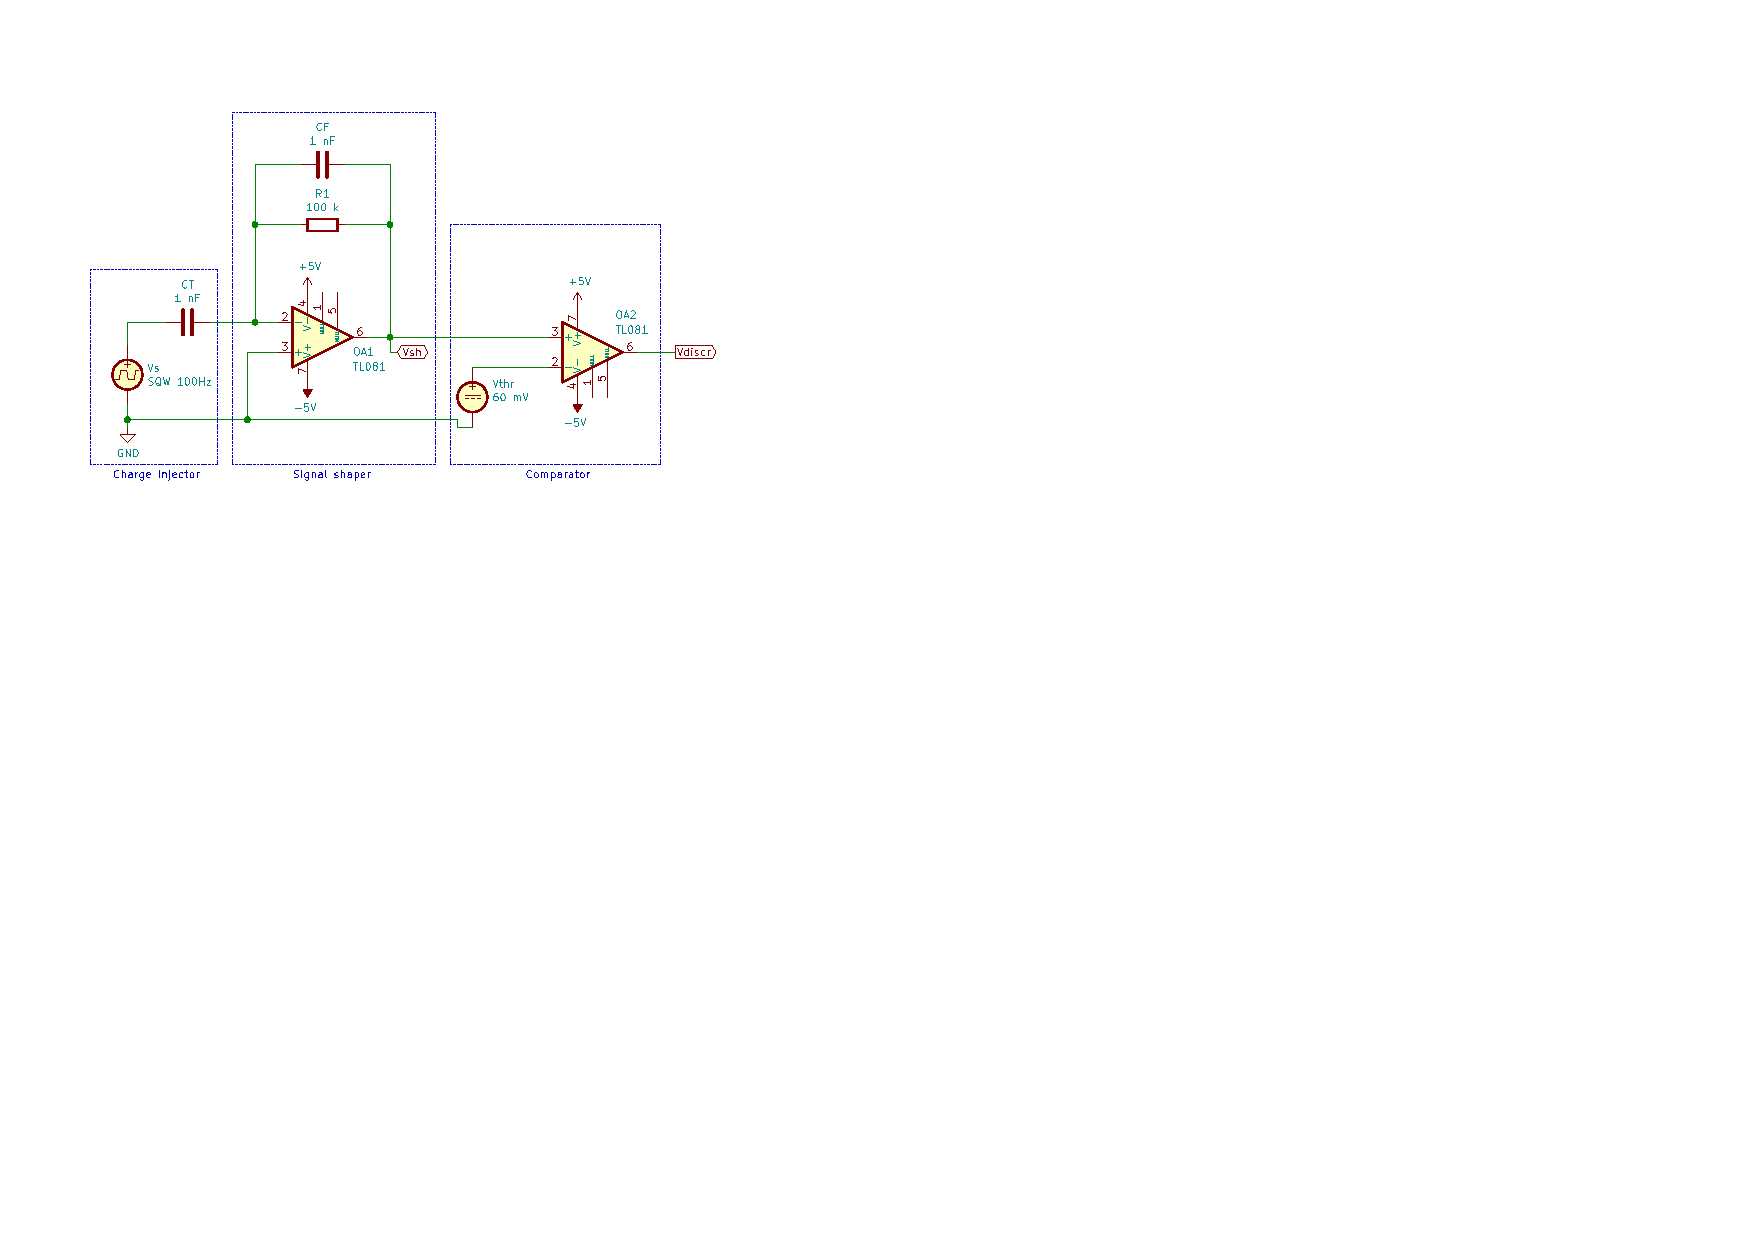
\includegraphics[scale=1.2]{Qamp}
    \caption{Schema circuitale dell'amplificatore di carica costruito.
    \label{fig: Qampschm}}
\end{figure}

In condizione di op-amp ideale gli ingressi $+, -$ sono dei circuiti aperti,
per cui la stessa corrente scorre attraverso $R_1$ ed $R_2$:
$V_+ = V_- \approx 0$.
Questo implica che
\begin{equation}\label{eq: Zin}
R\ped{in} \approx R_1
\end{equation}
allora per soddisfare la richiesta $5 \leq A_v \leq 10$ basta imporre
$5 R_1 \leq R_2 \leq 10 R_1$.

Dunque una volta fissata $R_1 = 1 \pm 1\% \; \si{k\ohm}$, dobbiamo avere
$\SI{5}{k\ohm} \leq R_2 \leq \SI{10}{k\ohm}$, di conseguenza scegliamo
$R_2 = 5.1 \pm 1\% \; \si{k\ohm}$, che corrisponde ad un guadagno
di centro banda $A\ped{v, atteso} = 5.1 \pm 2\%$ 

\subsection{Amplificazione di piccoli segnali}
Si è inviato all'ingresso di entrambi i circuiti un segnale sinusoidale di
ampiezza $v\ped{in} = 200 \pm 2 \; \si{m\V}$ ad una frequenza fissata
$5.01 \pm 0.05 \; \si{k\Hz}$.

Dunque abbiamo misurato l'ampiezza del segnale in uscita dal circuito con
$R_2^a = \SI{5.1}{k\ohm}$, che risulta $v\ped{out} = 1022 \pm 8 \; \si{m\V}$,
ottenendo così una stima del guadagno dell'amplificatore
$A_v = \dfrac{v\ped{out}}{v\ped{in}} = 5.11 \pm 0.06 $.

Consideriamo il sotto-circuito formato dal condensatore $ C\ped{T} $ e dal 
circuito di formazione. La funzione di trasferimento che lega $ 
V\ped{in} $ a $ V\ped{sh} $ è data di fatto da quella di un amplificatore 
invertente con impedenze complesse: in trasformata di Laplace
\[
\tilde{A}(s) = - \frac{\left(\frac{1}{R_{1}} + s 
C\ped{F}\right)^{-1}}{\frac{1}{s C\ped{T}}} = - \frac{C\ped{T}}{C\ped{F}} 
\frac{s}{s + \frac{1}{\tau}}
\]
con $ \tau \coloneqq R_{1} C\ped{F} $. In ingresso abbiamo un'onda quadra di 
periodo $ 2T $ (che prendiamo nulla per tempi negativi) che possiamo scrivere 
come
\[
V\ped{in}(t) = \sum_{k=0}^{+\infty} (-1)^{k}f(t - kT)
\qquad \text{dove} \quad
f(t) = V_{0} \left[\theta(t) - \theta(t - T)\right]
\]
In trasformata di Laplace si ha
\[
\tilde{f}(s) = V_{0}\left[\frac{1}{s} - \frac{e^{-sT}}{s}\right]
\]
da cui
\[
\tilde{V}\ped{in}(s) = \sum_{k=0}^{+\infty} (-1)^{k} \tilde{f}(s) e^{-kTs} = 
\tilde{f}(s) \sum_{k=0}^{+\infty} (-1)^{k} e^{-kTs}
\]
La risposta del circuito in trasformata è
\[
  \tilde{V}\ped{sh}(s) = \tilde{A}(s) \tilde{V}\ped{in}(s) =  
\tilde{A}(s)\tilde{f}(s) \sum_{k=0}^{+\infty} (-1)^{k}e^{-kTs} = \tilde{g}(s) 
\sum_{k=0}^{+\infty} (-1)^{k}e^{-kTs} = \mathcal{L}\left[\sum_{k=0}^{+\infty} 
(-1)^{k}g(t - kT)\right](s)
\]
Ora
\[
  \tilde{g}(s) = - V_{0} \frac{C\ped{T}}{C\ped{F}} \left[\frac{1}{s + 
\frac{1}{\tau}} - \frac{e^{-sT}}{s + \frac{1}{\tau}}\right]
\]
da cui, anti-trasformando
\[
  g(t) = - V_{0} \frac{C\ped{T}}{C\ped{F}} \left[e^{-t/\tau}\theta(t) - 
e^{-(t-T)/\tau} \theta(t - T) \right]
\]

Ma allora la risposta del circuito nel dominio del tempo è
\begin{align*}
  V\ped{sh}(t) &= - V_{0} \frac{C\ped{T}}{C\ped{F}} \left\{ 
\sum_{k=0}^{+\infty} (-1)^{k}e^{-\frac{t - kT}{\tau}}\theta(t - kT) - 
\sum_{k=0}^{+\infty} (-1)^{k} e^{-\frac{t- (k+1) T }{\tau}} \theta(t - (k+1)T ) 
\right\} \\
               &= - V_{0} \frac{C\ped{T}}{C\ped{F}} \left\{ e^{-\frac{t}{\tau}} 
\theta(t) - 2 \sum_{k=1}^{+\infty} (-1)^{k} e^{-\frac{t - kT}{\tau}} \theta(t - 
kT) \right\}
\end{align*}
ovvero, ignorando il transiente iniziale e supponendo $ \tau\ll T $\footnote{
La buona definizione della somma è assicurata dal fatto che (tralasciando le 
costanti fisiche)
\[ \sum_{k \geq 0} \theta(t-k) e^{-(t-k)} = \sum_{k=0}^{\lfloor t \rfloor} 
e^{-(t-k)} \leq \frac{e}{e-1} e^{-\{t\}}. \]
},
\begin{align}\label{eq:Vsh}
V\ped{sh}(t) &\approx 2 V_{0} \frac{C\ped{T}}{C\ped{F}} \sum_{k=1}^{+\infty} 
(-1)^{k} e^{-\frac{t - kT}{\tau}} \theta(t - kT) \nonumber\\
               &\approx  2 V_{0} \frac{C\ped{T}}{C\ped{F}} \sum_{k=1}^{+\infty} 
(-1)^{k} e^{-\frac{t - kT}{\tau}} \chi_{[kT, (k+1)T]}(t)
\end{align}
Per il circuito in esame i valori nominali sono $ C\ped{T} = C\ped{F} = 
\SI{1}{\nano\farad} $, $ R_{1} = \SI{100}{\kilo\ohm} $, da cui $ \tau = 
\SI{100}{\micro\second} $, e $ 2T = \SI{10}{\milli\second} $. Dopo un 
transiente $ t\ll\tau $ in uscita ci aspettiamo quindi di osservare dei picchi 
esponenzialmente decrescenti di segno alterno e di ampiezza pari al doppio del 
segnale in ingresso. \\

\paragraph{Discriminatore}
Ignorando ora il condensatore $ C_{1} $ che ha il solo scopo di rimuovere il 
rumore ad alte frequenze dal generatore, il sotto-circuito \texttt{X2} è un 
discriminatore con tensione di soglia $ V\ped{t} $ data dal partitore di 
tensione collegato al terminale ``--'' dell'OpAmp
\[
  V\ped{t} = (1 - 2\alpha) V\ped{G}
\]
dove $ 0\leq \alpha \leq 1 $ è la ``frazione'' di resistenza data dal 
potenziometro e $ V\ped{G} = \SI{15}{\volt} $ (valore nominale) è la tensione 
di alimentazione. In altri termini la tensione di soglia è variabile da $ 
\SI{-15}{\volt} $ a $ \SI{15}{\volt} $. Supponendo di essere sempre in regime 
di saturazione, l'uscita del circuito è data da
\[
  V\ped{out} = V\ped{G} \sgn\left(V\ped{sh} - V\ped{t}\right).
\]
Più esplicitamente, usando $ V\ped{in} = \SI{6}{\volt} $ ci aspettiamo $ 
V\ped{sh} = \SI{12}{\volt} $ (ampiezze picco-picco), pertanto:
\begin{itemize}
\item se $ V\ped{t} > \SI{6}{\volt} $, $ V\ped{out} = -V\ped{G} $ costante.
\item se $ \SI{0}{\volt} < V\ped{t} < \SI{6}{\volt} $, ci aspettiamo (in un 
periodo)
  \[
    V\ped{out}(t) =
    \begin{cases}
      V\ped{G} & 0 < t < h \\
      - V\ped{G} & h < t < 2T
    \end{cases}
  \]
  dove $ h $ è il tempo in cui il picco esponenzialmente decrescente è 
maggiore della tensione di soglia, ovvero
  \begin{equation} \label{eq:tot-ampiezza-durata}
    h = \tau \log\left(\frac{C\ped{F}}{C\ped{T}} 
\frac{V\ped{in}}{V\ped{t}}\right).
  \end{equation}
\item se $ \SI{-6}{\volt} < V\ped{t} < \SI{0}{\volt} $, ci aspettiamo (in un 
periodo)
  \[
    V\ped{out}(t) =
    \begin{cases}
      V\ped{G} & 0 < t < T \\
      - V\ped{G} & T < t < T + h' \\
      V\ped{G} & T + h' < t < 2T
    \end{cases}
  \]
  dove $ h' $ è il tempo in cui il picco esponenzialmente crescente è minore 
della tensione di soglia, ovvero
  \[
    h' = \tau \log\left(\frac{C\ped{F}}{C\ped{T}} 
\frac{V\ped{in}}{\abs{V\ped{t}}}\right).
  \]
\item se $ V\ped{t} < \SI{-6}{\volt} $, $ V\ped{out} = -V\ped{G} $ costante.
\end{itemize}

\setcounter{subsection}{3}
\subsection{Misure di guadagno al variare di $v\ped{in}$}
Misurando con l'oscilloscopio l'ampiezza dei segnali in ingresso $v\ped{in}$
e in uscita $v\ped{out}$ dall'amplificatore possiamo ricavare una misura del
guadagno del circuito dal rapporto $A_v = \dfrac{v\ped{out}}{v\ped{in}}$.

\begin{table}[htbp]
\centering
\begin{tabular}{cccc}
\toprule
$v\ped{in}(\si{m\V})$ (nom.) & $v\ped{in} \pm \sigma(v\ped{in})$ [mV] & 
$v\ped{out} \pm \sigma(v\ped{out})$ [V] & $A_v \pm \sigma(A_v)$ \\
\midrule
\midrule
40 & $40.1 \pm 0.2$ & $283 \pm 1.7 \; \si{m}$ & $7.06 \pm 0.06$ \\
60 & $59.8 \pm 0.3$ & $410 \pm 2 \; \si{m}$ & $6.86 \pm 0.06$ \\
80 & $79.9 \pm 1.1$ & $564 \pm 3 \; \si{m}$ & $7.06 \pm 0.06$ \\
100 & $100.1 \pm 1.2$ & $705 \pm 4 \; \si{m}$ & $7.04 \pm 0.06$ \\
200 & $200 \pm 2$ & $1412 \pm 8 \; \si{m}$ & $7.06 \pm 0.06$ \\
400 & $401 \pm 3$ & $2882 \pm 17 \; \si{m}$ & $7.04 \pm 0.06$ \\
600 & $601 \pm 5$ & $4.24 \pm 0.02$ & $7.05 \pm 0.06$ \\
800 & $801 \pm 6$ & $5.78 \pm 0.03$ & $7.21 \pm 0.06$ \\
900 & $900 \pm 6$ & $6.32 \pm 0.04$ & $7.00 \pm 0.06$ \\
1000 & $1000 \pm 7$ & $7.04 \pm 0.04$ & $7.02 \pm 0.06$ \\
\bottomrule
\end{tabular} 
\caption{Misure di guadagno al variare della tensione in ingresso
all'amplificatore con $R_2^a = \SI{7}{k\ohm}$. Le ampiezze per questo
circuito sono riportate per comodità in ampiezza picco-picco. A partire
da valori di ampiezza (picco-picco) di \SI{1}{\V} del segnale in ingresso la
parte inferiore dell'onda in uscita viene ``tosata''. \label{tab: gain_M}}
\end{table}

Con un fit lineare possiamo stimare il guadagno dell'amplificatore a partire
dal grafico di $v\ped{out} = A_v v\ped{in}$ al variare di $v\ped{in}$.
Riportiamo quanto trovato per il primo circuito:
\begin{figure}[htbp]
\centering
%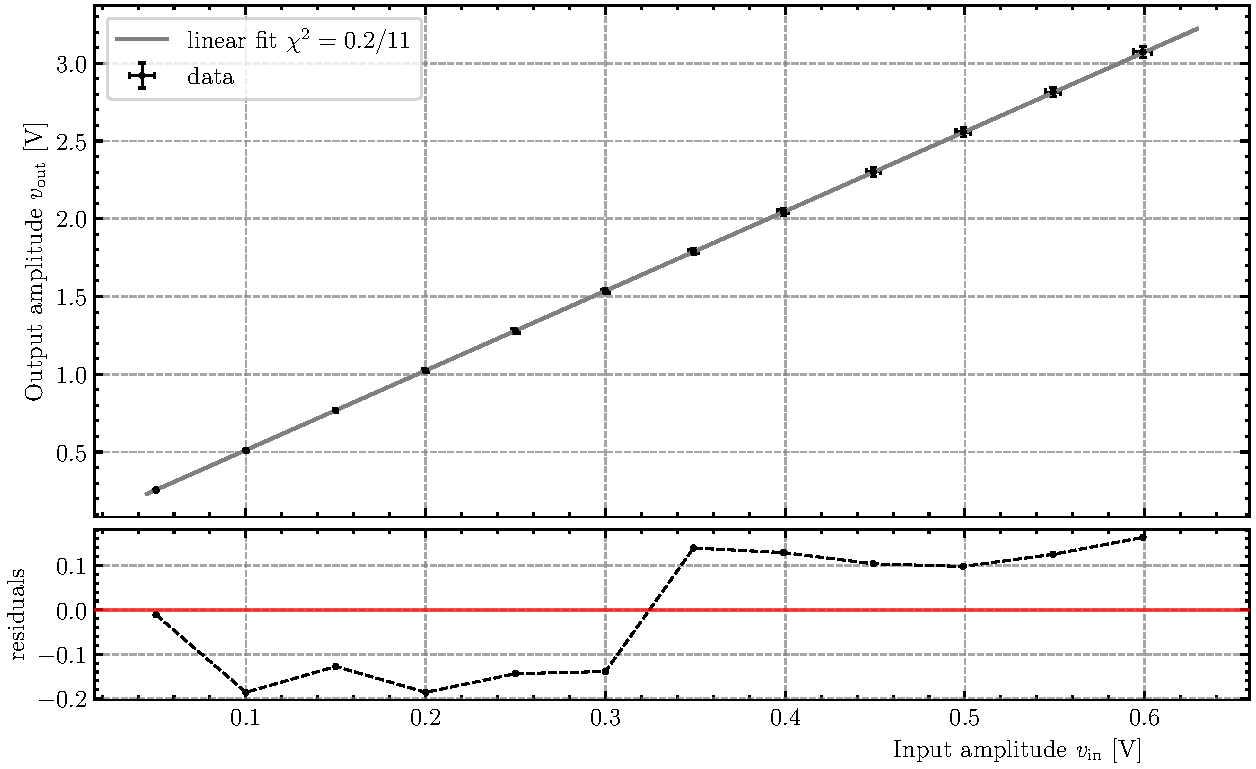
\includegraphics[scale=0.7]{gain5k1}
\caption{Fit lineare per l'andamento dell'uscita rispetto al segnale in
ingresso. \label{fig: gainfit}}
\end{figure}
Da cui troviamo i seguenti parametri per la retta di best-fit
\begin{align*}
\mathrm{intercetta} = -0.6 \pm 0.4 \; \si{m\V} \;\;\;\mathrm{pendenza} = 5.124 
\pm 0.003 \;\;\;\mathrm{correlazione} 
= -0.72 \;\;\; \chi^2 = 0.2 \;\;\; d.o.f. = 10 \\
\text{coefficiente angolare/senza intercetta} = 5.120 \pm 0.002 \;\;\;
\chi^2 = 0.2 \;\;\; d.o.f. = 11
\end{align*}

Il valore atteso per il guadagno dal valore dei componenti in questa
configurazione del circuito è pari a
\[
A\ped{v, exp} = -\frac{R_2}{R_1} = - 5.13 \pm 0.12
\]
Questo è in ottimo accordo con quanto trovato sperimentalmente dalla nostra
analisi.

Per completezza riportiamo in un grafico anche le misure che non abbiamo
considerato nel fit perché oltre la regione in cui l'op-amp ha comportamento
lineare
\begin{figure}[htbp]
\centering
%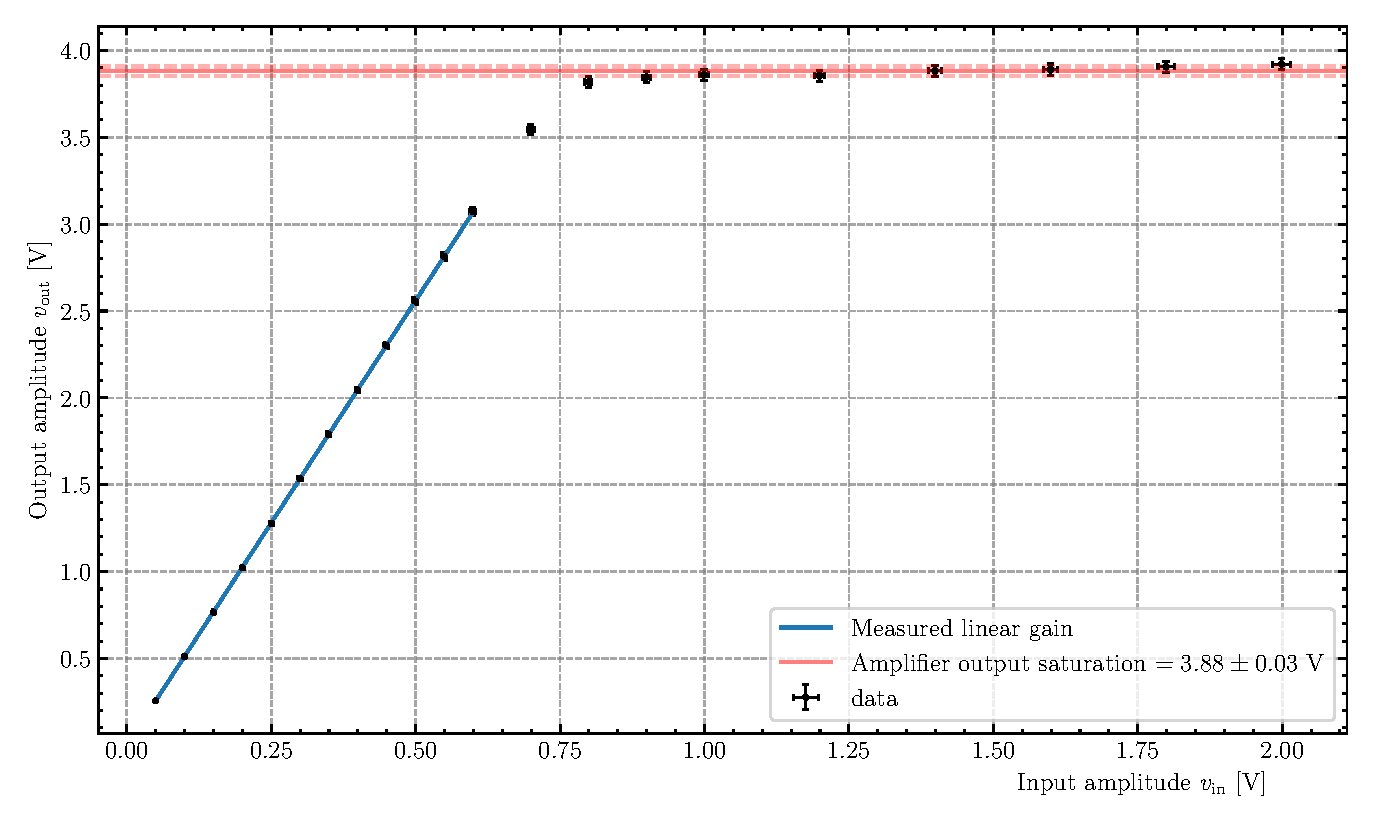
\includegraphics[scale=0.7]{gainsat}
\caption{Andamento reale dell'uscita al variare dell'ampiezza del segnale in
ingresso oltre il regime lineare dell'amplificatore misurati per il circuito
con $R_2^a = 5.1 \; \si{k\ohm}$ \label{fig: gainsat}}
\end{figure}

\subsection{Durata impulso per carica di test}
Abbiamo misurato per $V_s = 999 \pm 8 \si{m\V}$ di ampiezza dell'onda quadra
in ingresso, frequenza $f = 100.0 \pm 1.6 \; \si{k\Hz}$, dunque come carica
$Q\ped{in} = C_T \cdot V_s = 0.99 \pm 0.04 \; \si{n\coulomb}$.

L'impulso in uscita ha durata pari a $415 \pm 5 \; \si{\micro\s}$.

\subsection{Andamento di TOT al variare di $Q\ped{in}$}
\begin{table}[htbp]
\centering
\begin{tabular}{cccc}
\toprule
$v\ped{in}(\si{m\V})$ (nom.) & $v\ped{in} \pm \sigma(v\ped{in})$ [mV] & 
$v\ped{out} \pm \sigma(v\ped{out})$ [V] & $A_v \pm \sigma(A_v)$ \\
\midrule
\midrule
50 & $50.0 \pm 0.4$ & $256 \pm 2 \; \si{m}$ & $5.12 \pm 0.06$ \\
100 & $100.0 \pm 0.8$ & $511 \pm 4 \; \si{m}$ & $5.11 \pm 0.06$ \\
150 & $150.0 \pm 1.2$ & $767 \pm 6$ & $5.11 \pm 0.06$ \\
200 & $200 \pm 1.6$ & $1022 \pm 8$ & $5.11 \pm 0.06$ \\
250 & $250 \pm 2$ & $1278 \pm 11$ & $5.11 \pm 0.06$ \\
300 & $300 \pm 2$ & $1534 \pm 12$ & $5.11 \pm 0.05$ \\
350 & $349 \pm 3$ & $1790 \pm 14$ & $5.13 \pm 0.06$ \\
400 & $399 \pm 3$ & $2046 \pm 16$ & $5.13 \pm 0.06$ \\
450 & $449 \pm 4$ & $2302 \pm 18$ & $5.13 \pm 0.06$ \\
500 & $499 \pm 4$ & $2.56 \pm 0.02$ & $5.13 \pm 0.06$ \\
550 & $549 \pm 4$ & $2.82 \pm 0.02$ & $5.13 \pm 0.06$ \\
600 & $599 \pm 5$ & $3.07 \pm 0.02$ & $5.13 \pm 0.06$ \\
\\
700 & $699 \pm 6$ & $3.55 \pm 0.03$ & $5.07 \pm 0.06$ \\
800 & $799 \pm 6$ & $3.82 \pm 0.03$ & $4.78 \pm 0.05$ \\
900 & $899 \pm 7$ & $3.86 \pm 0.03$ & $4.28 \pm 0.05$ \\
1 V & $999 \pm 8$ & $3.86 \pm 0.03$ & $3.86 \pm 0.04$ \\
1.2 V & $1199 \pm 9$ & $3.86 \pm 0.03$ & $3.22 \pm 0.04$ \\
1.4 V & $1399 \pm 11$ & $3.88 \pm 0.03$ & $2.78 \pm 0.03$ \\
1.6 V & $1599 \pm 12$ & $3.89 \pm 0.03$ & $2.43 \pm 0.03$ \\
1.8 V & $1799 \pm 14$ & $3.90 \pm 0.03$ & $2.17 \pm 0.02$ \\
2 V & $1999 \pm 15$ & $3.92 \pm 0.03$ & $1.96 \pm 0.02$ \\
\bottomrule
\end{tabular} 
\caption{Misure di guadagno al variare della tensione in ingresso
all'amplificatore con $R_2^a = 5.1 \; \si{k\ohm}$. Oltre i \SI{600}{m\V} di
ampiezza del segnale in ingresso la forma d'onda in uscita inizia a
manifestare difetti dovuti al clipping dell'op-amp al di fuori del regime
lineare. \label{tab: gain_B}}
\end{table}

Per 40 mV l'impulso si deforma in una parabola
Sotto i 20 mV non c'è segnale apprezzabile in uscita.

%=======================
\section{Trigger di Schmitt}

\begin{figure}[htbp]
    \centering
	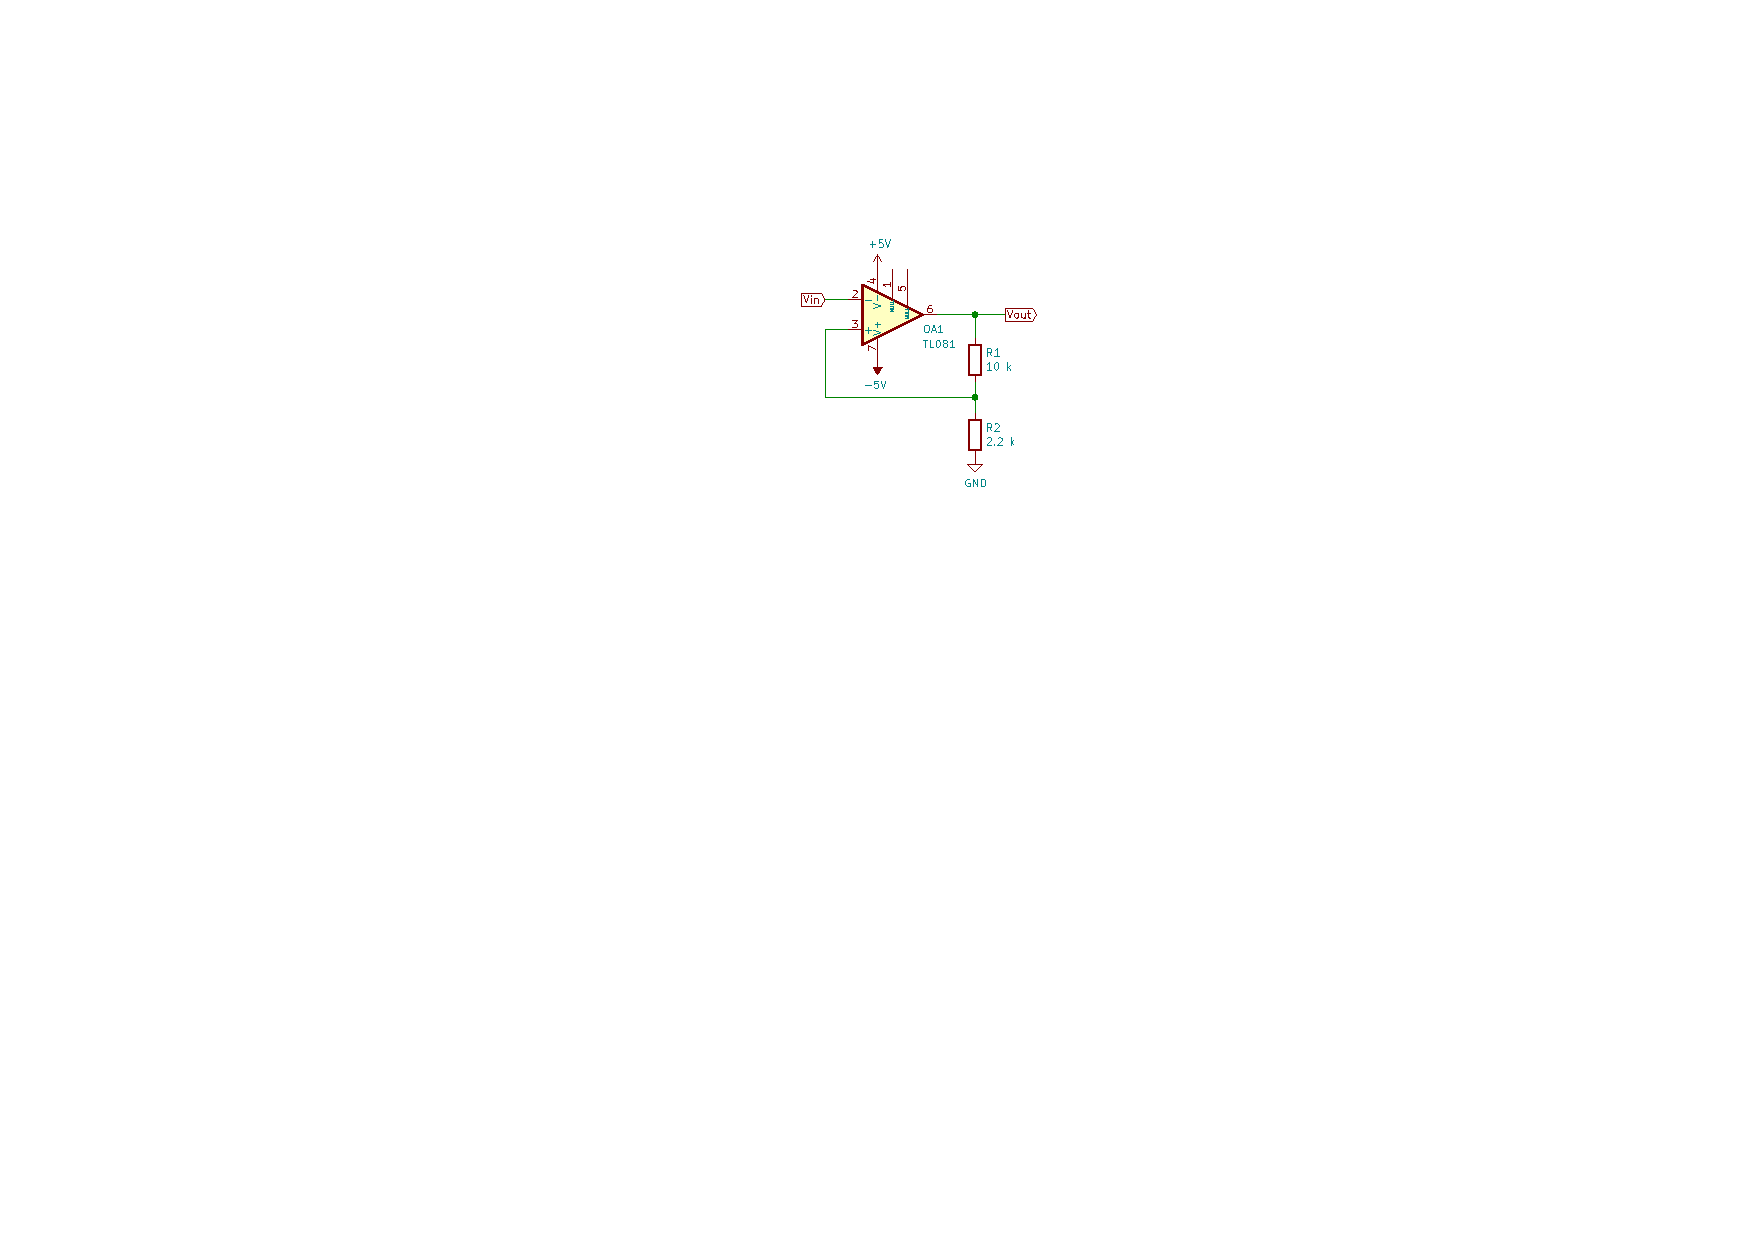
\includegraphics[scale=1.5]{trgSchmitt}
    \caption{Schema circuitale del trigger di Schmitt costruito.
    \label{fig: trgschmittschm}}
\end{figure}

\subsection{Risposta ad un'onda sinusoidale}
Con l'aiuto dei cursori abbiamo misurato come guadagno a centro banda
per il circuito amplificatore con resistenza $R_2^a = 5.1 \; \si{k\ohm}$
$A_M = 14.18 \pm 0.09 \; \si{dB} = 5.12 \pm 0.05$
dunque abbiamo ricavato una stima della frequenza di taglio dell'amplificatore
invertente dal punto in cui il guadagno diminuisce di $-3.01 \; \si{dB}$
rispetto ad $A_M$:
$f_A = 388.0 \pm 1.1 \; \si{k\Hz}$
\begin{figure}[htbp]
\centering
%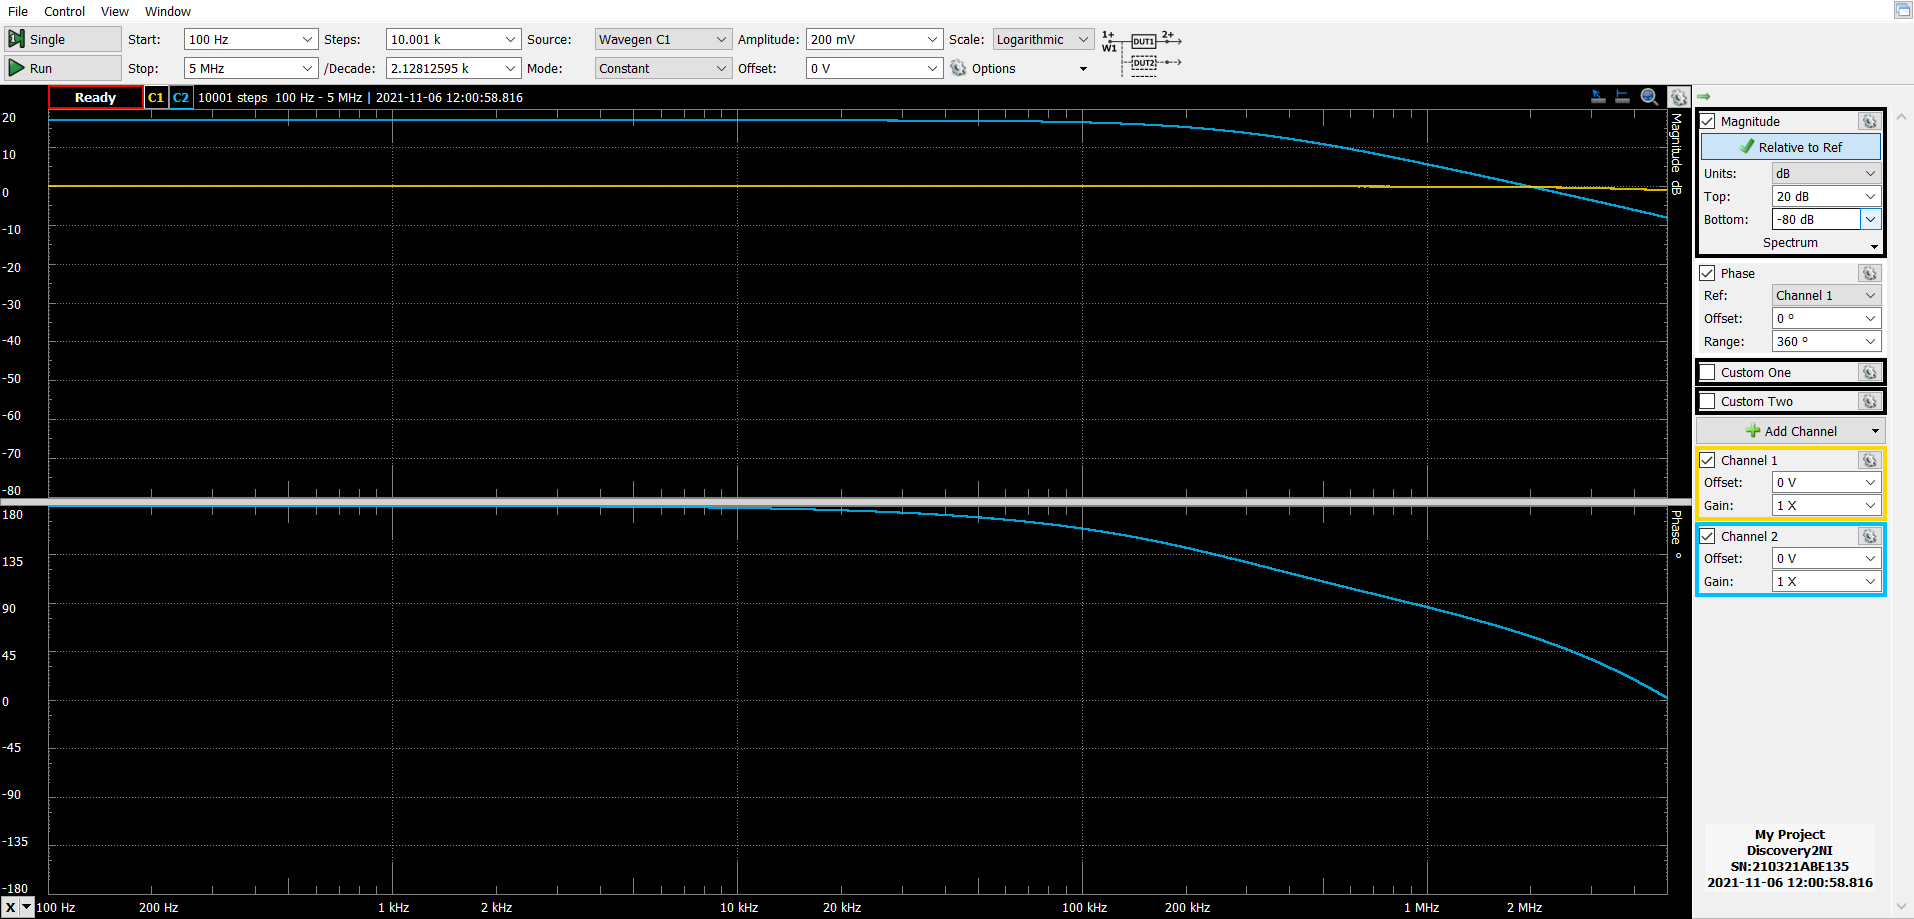
\includegraphics[scale=0.4]{opampbode}
\caption{Plot di Bode ottenuto dallo scan con Network tra $\SI{100}{\Hz}$ e
$\SI{5}{M\Hz}$ con un segnale sinusoidale in ingresso all'amplificatore
invertente di ampiezza costante $v\ped{in} = \SI{200}{m\V}$. \label{fig: 
invbode}}
\end{figure}

Per caratterizzare le frequenze di taglio misurate possiamo ricavare un valore
atteso con cui confrontarle a partire dal valore del prodotto banda guadagno
(GBW) riportato nel datasheet dell'op-amp: $\SI{4}{M\Hz}$\footnote{Assumendo
che il prodotto banda-guadagno sia costante, come frequenza di taglio
attesa in funzione del guadagno dell'amplificatore abbiamo
$f\ped{A, exp} = \mathrm{GBW}/A_v$}.

\subsection{Saturazione dell'OpAmp}
Abbiamo inviato in ingresso all'amplificatore un'onda sinusoidale di ampiezza
$1999 \pm 15 \; \si{m\V}$ e frequenza $1000 \pm 16 \; \si{\Hz}$.
Dalle intersezioni tra i due canali abbiamo misurato le transizioni basso-alto
(OH) e alto-basso (OL)

\[
V_{OH} = 617 \pm 5 \; \si{m\V}
V_{OL} = 782 \pm 6 \; \si{m\V}
\]

Misurando con l'oscilloscopio di quanto sale la tensione in uscita
dall'amplificatore $\Delta V$ in un certo intervallo di tempo $\Delta t$
(presi su una porzione lineare della rampa) otteniamo una stima dello slew
rate dal loro rapporto; che rispettivamente per i circuiti con $R_2^a = 5.1$
e $7$ risulta
\begin{align*}
\mathrm{SR} = \frac{\Delta V}{\Delta t} =
\frac{6.19 \pm 0.04 \; \si{\V}}{542 \pm 10 \; \si{n\s}}
&= 11.4 \pm 0.2 \; \si{\V/\micro\s} \\
\mathrm{SR} = \frac{\Delta V}{\Delta t} =
\frac{4.10 \pm 0.04 \; \si{\V}}{354 \pm 10 \; \si{n\s}}
&= 11.6 \pm 0.3 \; \si{\V/\micro\s}  
\end{align*}

\begin{figure}[htbp]
\centering
%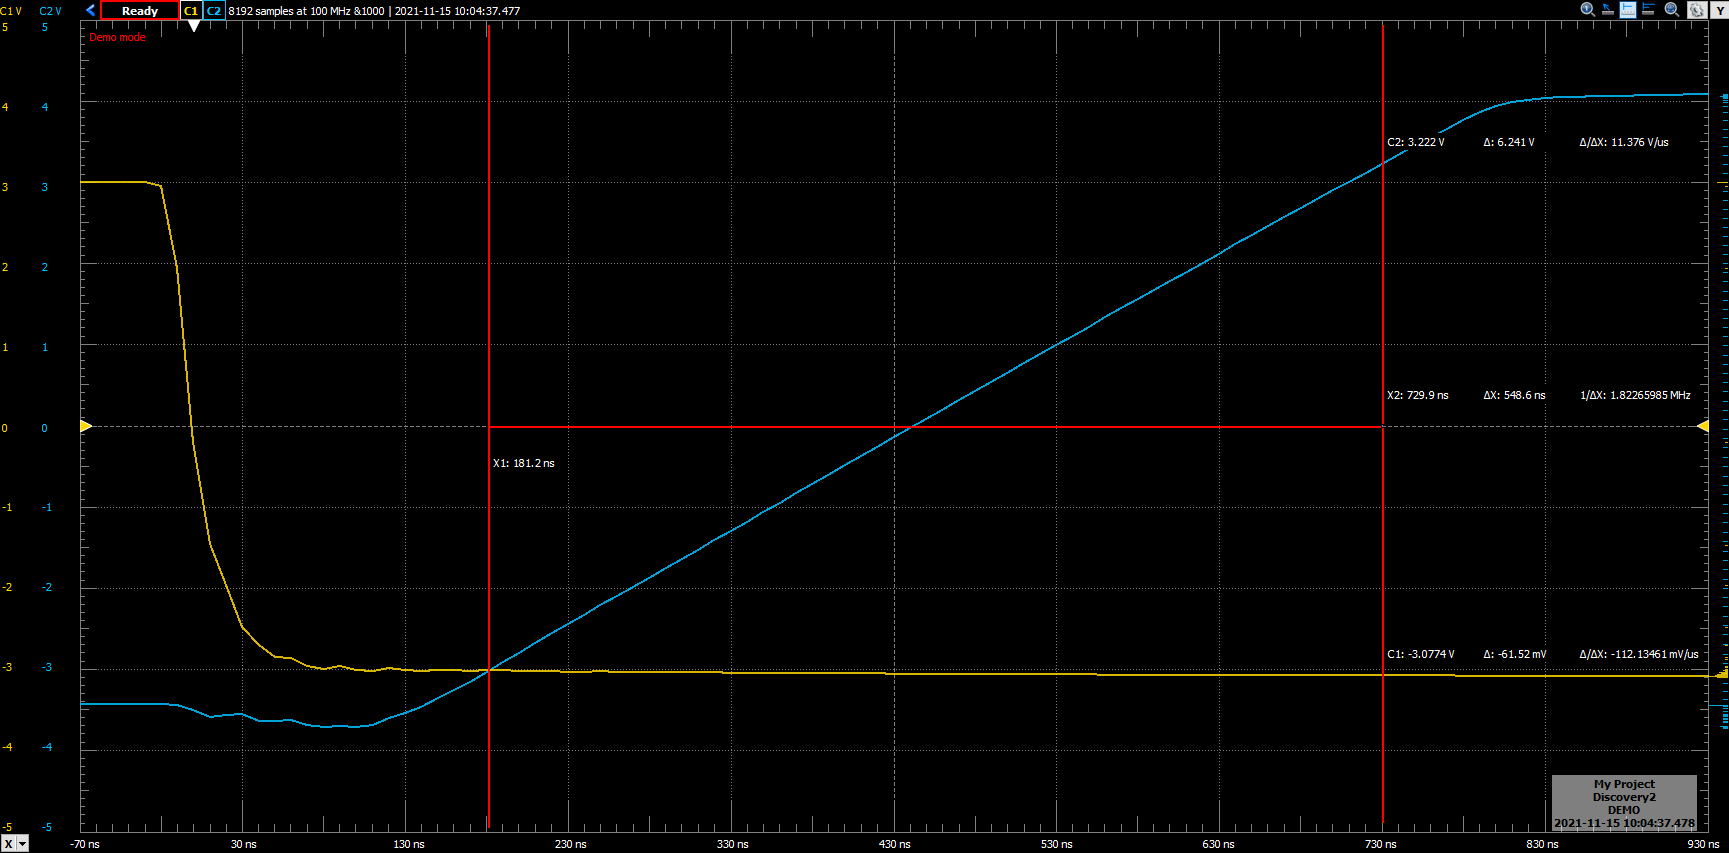
\includegraphics[scale=0.37]{slew}
\caption{La traccia della rampa in uscita dall'amplificatore visualizzata
all'oscilloscopio da cui abbiamo ottenuto la misura diretta dello slew rate.
\label{fig: slewrate}}
\end{figure}

\subsection{Tensioni di soglia e funzionamento del trigger}

\subsection{Limiti fisici del circuito}

%=======================
\section{Multivibratore astabile}

\begin{figure}[htbp]
    \centering
	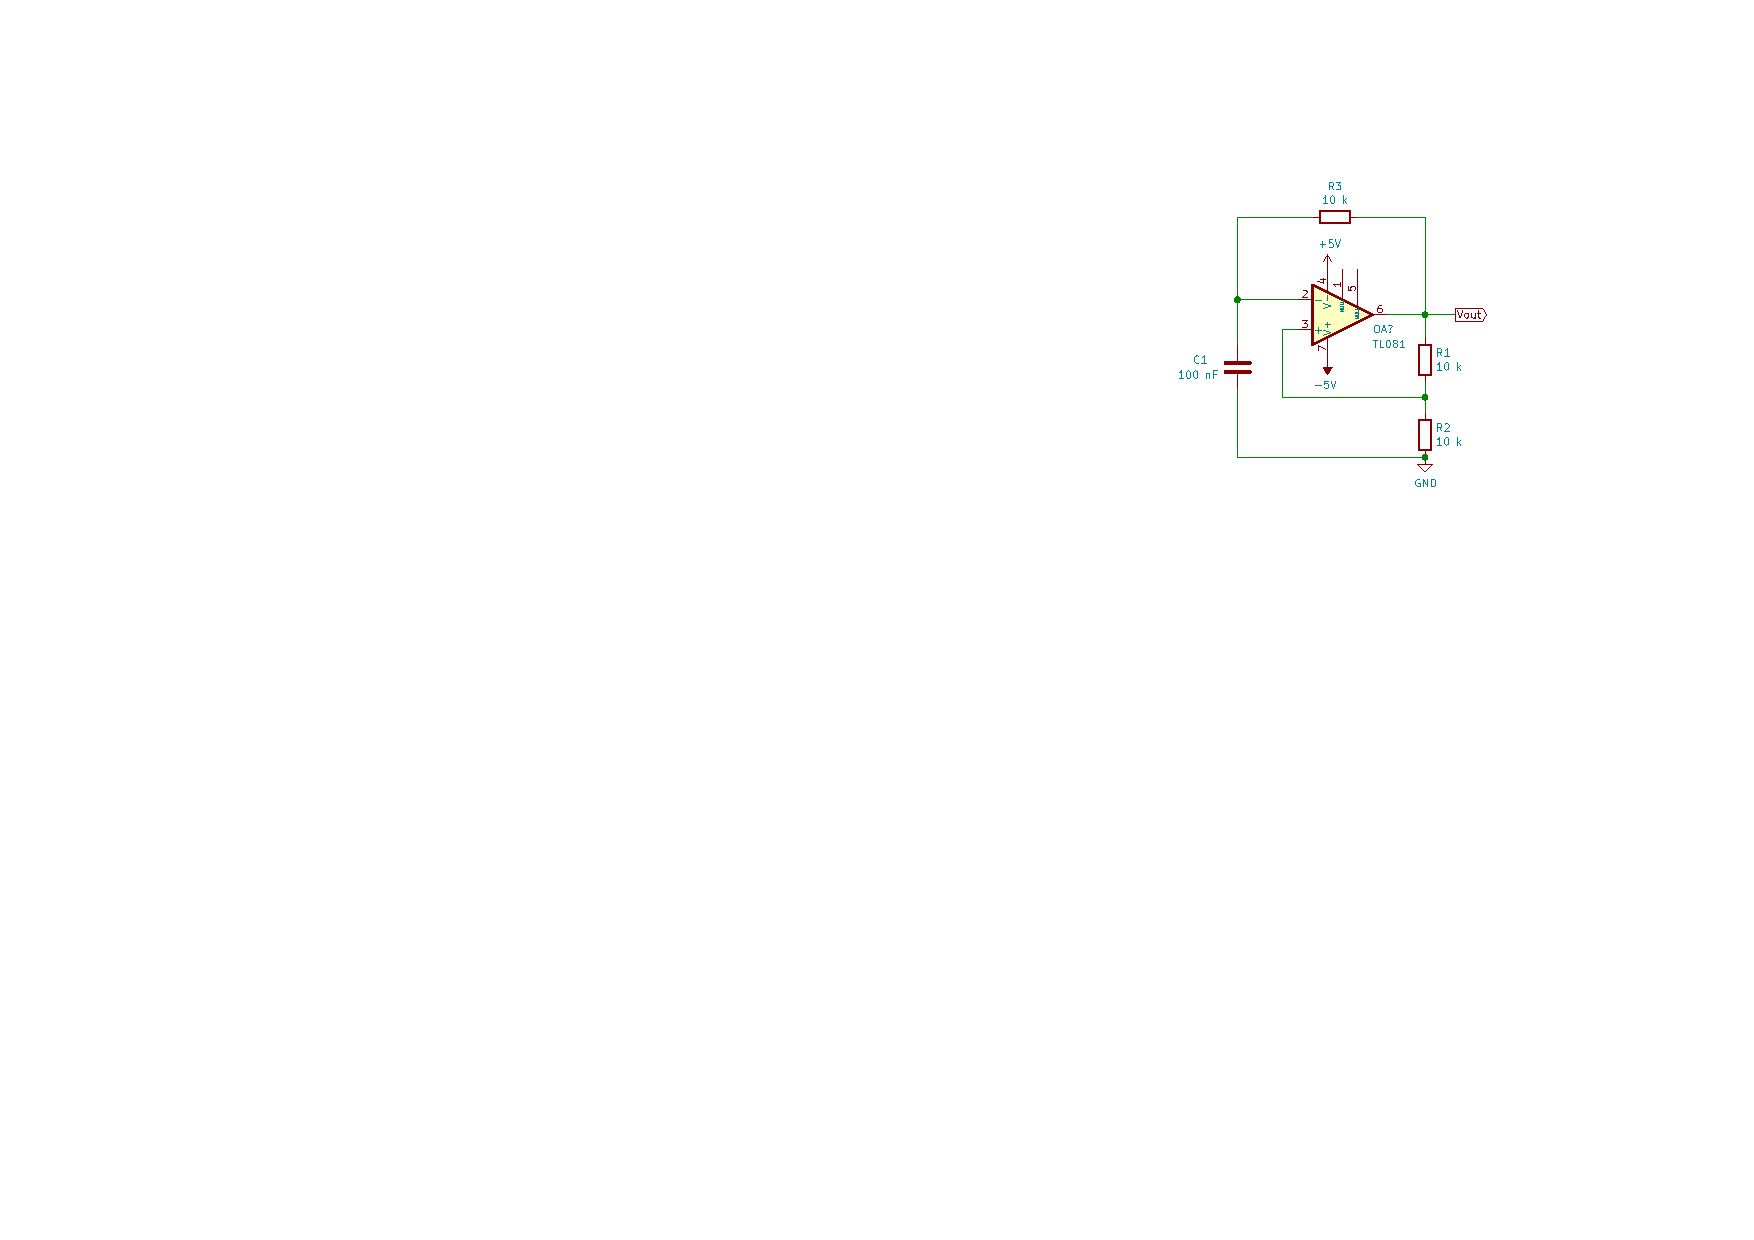
\includegraphics[scale=1.5]{astable}
    \caption{Schema circuitale del multivibratore astabile costruito.
    \label{fig: astableschm}}
\end{figure}

\subsection{Funzionamento del circuito}
Sempre usando i cursori abbiamo misurato come guadagno a centro banda
per i circuiti derivatori
\begin{align*}
A_M &= 20.02 \pm  0.09 \; \si{dB} \\
A_M &= 20.01 \pm  0.09 \; \si{dB}
\end{align*}

Dunque abbiamo ricavato una stima delle frequenze di taglio del circuito dai
due punti in cui il guadagno diminuisce di $-3.01 \; \si{dB}$ rispetto a
centro banda:
$f_c = 3408 \pm 11 \; \si{\Hz}$ e $f_A = 209 \pm 2 \; \si{k\Hz}$.
\begin{figure}[htbp]
\centering
%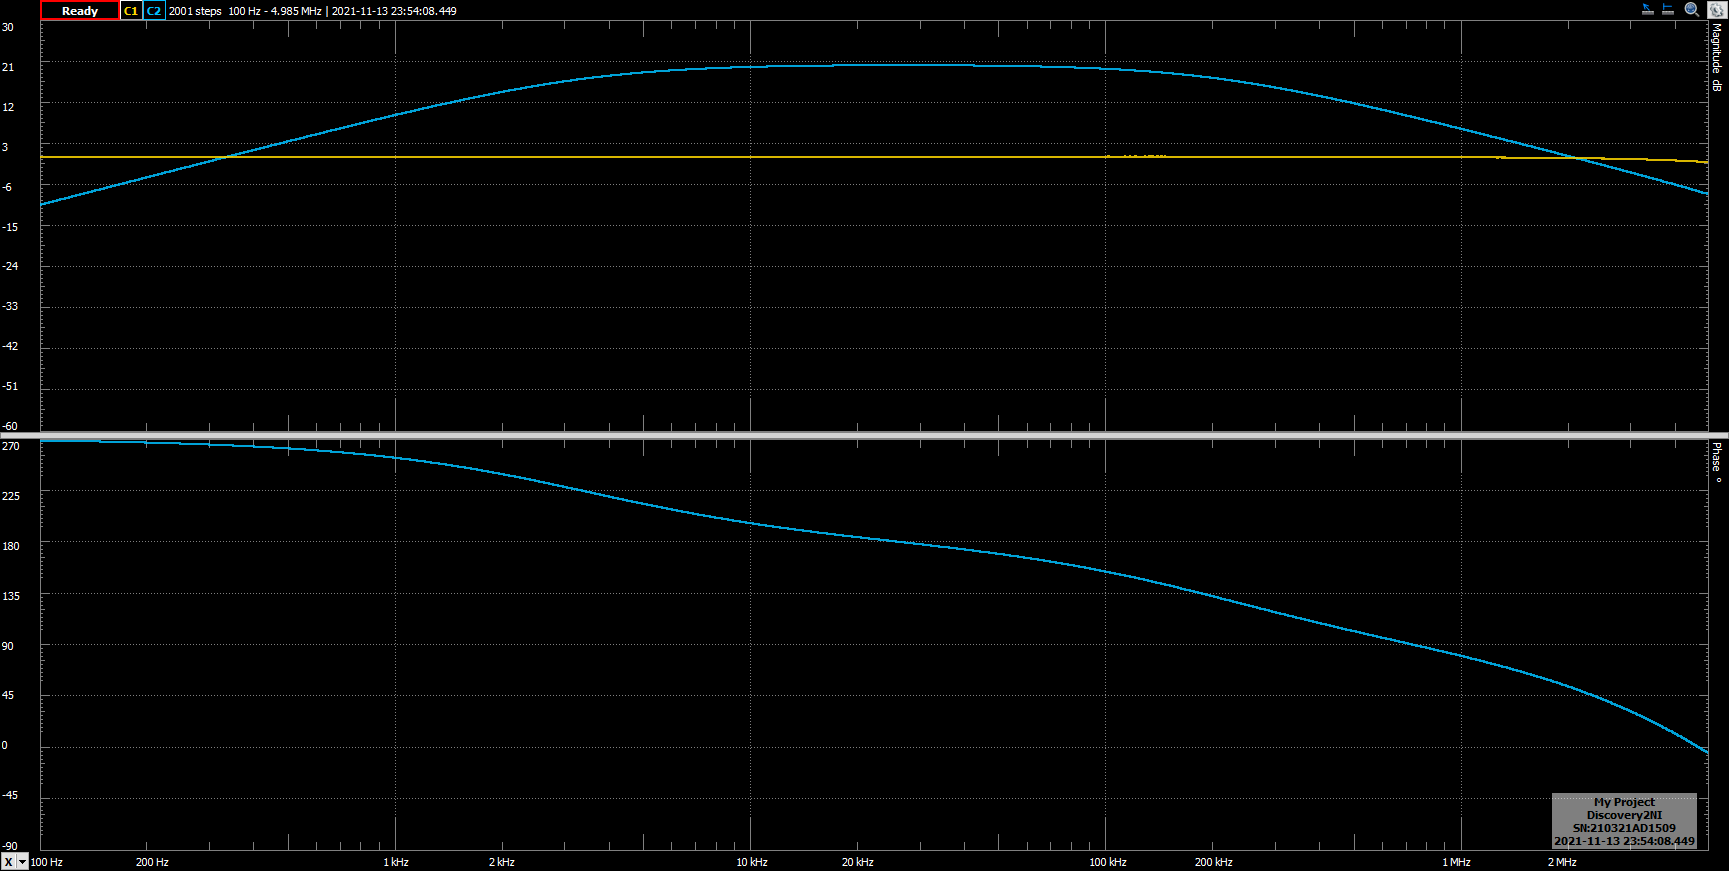
\includegraphics[scale=0.36]{hpfbode}
\caption{Plot di Bode ottenuto dallo scan con Network tra $\SI{100}{\Hz}$ e
$\SI{5}{M\Hz}$ con un segnale sinusoidale in ingresso al derivatore RC attivo
di ampiezza costante $v\ped{in} = \SI{200}{m\V}$.
\label{fig: derbode}}
\end{figure}

\setcounter{subsection}{2}
\subsection{Studio dei segnali in ingresso e uscita}
Si è inviato all'ingresso del filtro passa-alto un segnale triangolare di
ampiezza $v\ped{in} = 200 \pm 2 \si{m\V}$ e frequenza
$f = 100.0 \pm 1.6 \si{\Hz}$.

\begin{figure}[htbp]
\centering
%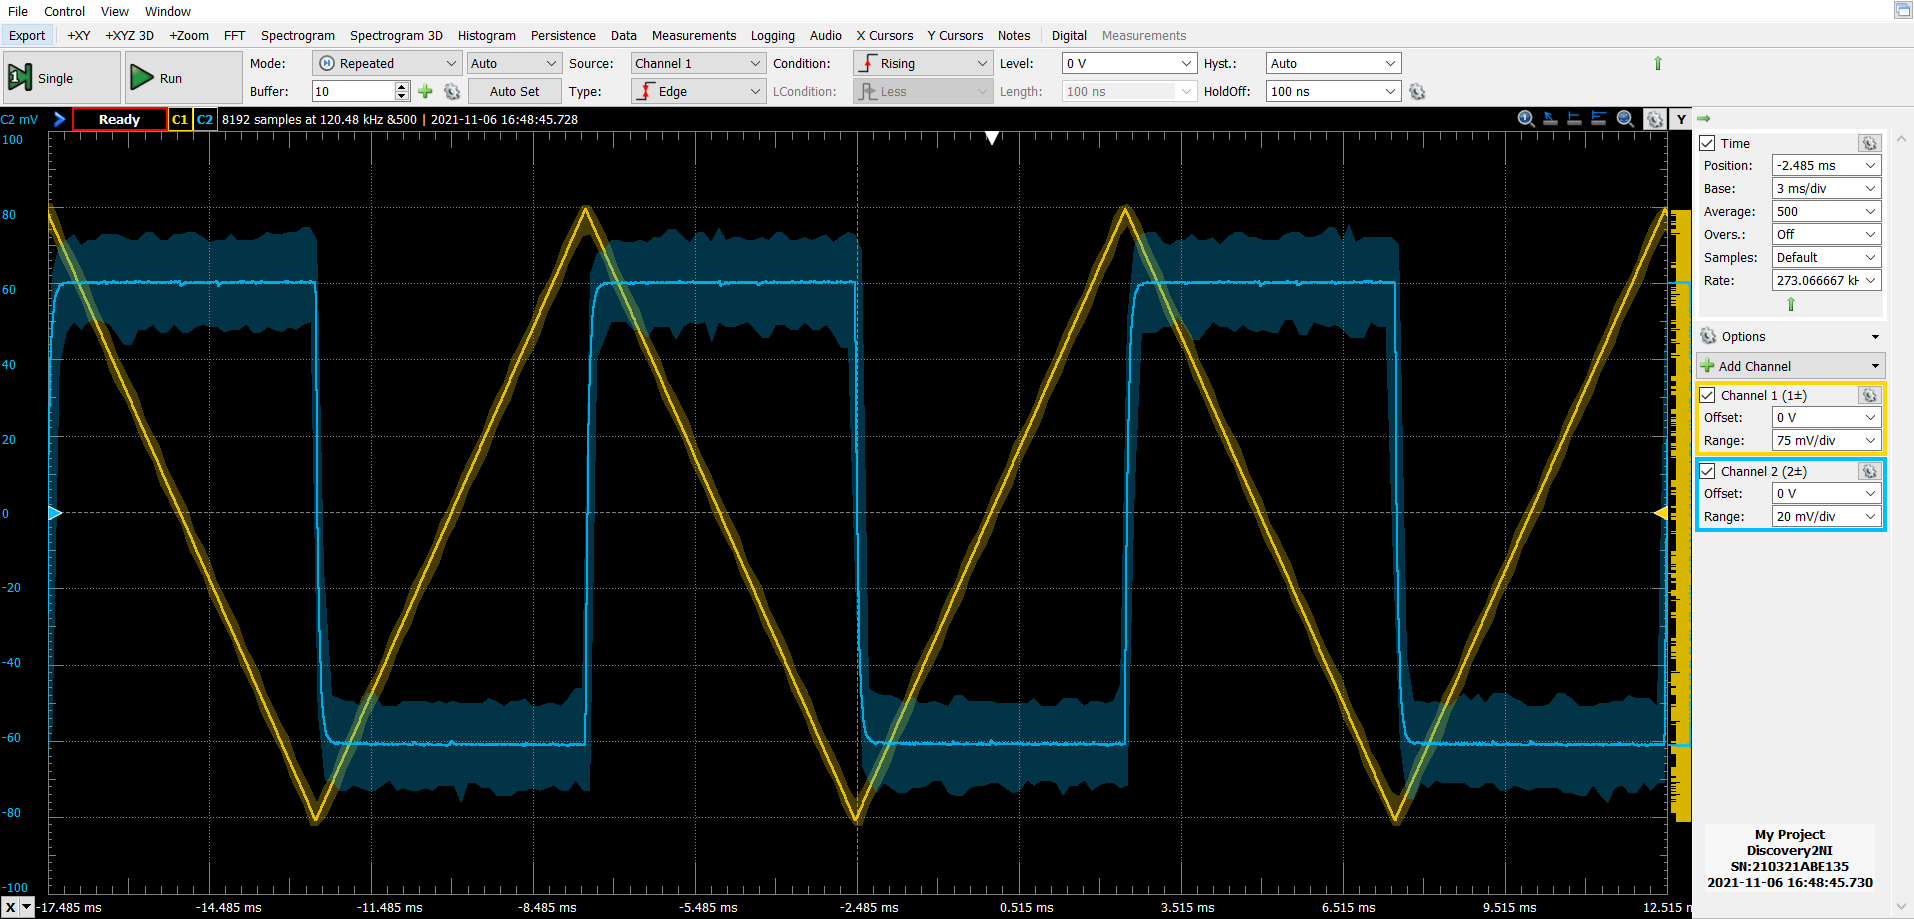
\includegraphics[scale=0.4]{derivatore}
\caption{Risposta del circuito ad un segnale triangolare di ampiezza
$\SI{200}{m\V}$ e $f = \SI{100}{\Hz}$ in ingresso. \label{fig: dertrg}}
\end{figure}

Per frequenze $f \ll f_c$ il filtro è in regime di taglio, per cui si comporta
come un derivatore, dunque la forma d'onda in uscita è un'onda quadra di
ampiezza sempre minore al diminuire della frequenza.

Per frequenze $f_c \ll f \ll f_A$ come ci si aspetta, la forma d'onda in uscita
rimane visivamente inalterata rispetto all'onda triangolare in ingresso,
che risulta però amplificata in ampiezza di un fattore $A_M \sim 10$.

Nel regime intermedio $f \sim f_c$ all'uscita del filtro RC osserviamo un'onda
"a pinna di squalo" caratteristica della carica e della scarica del
condensatore con cui abbiamo costruito il nostro filtro passa-alto.
\begin{figure}[htbp]
\centering
%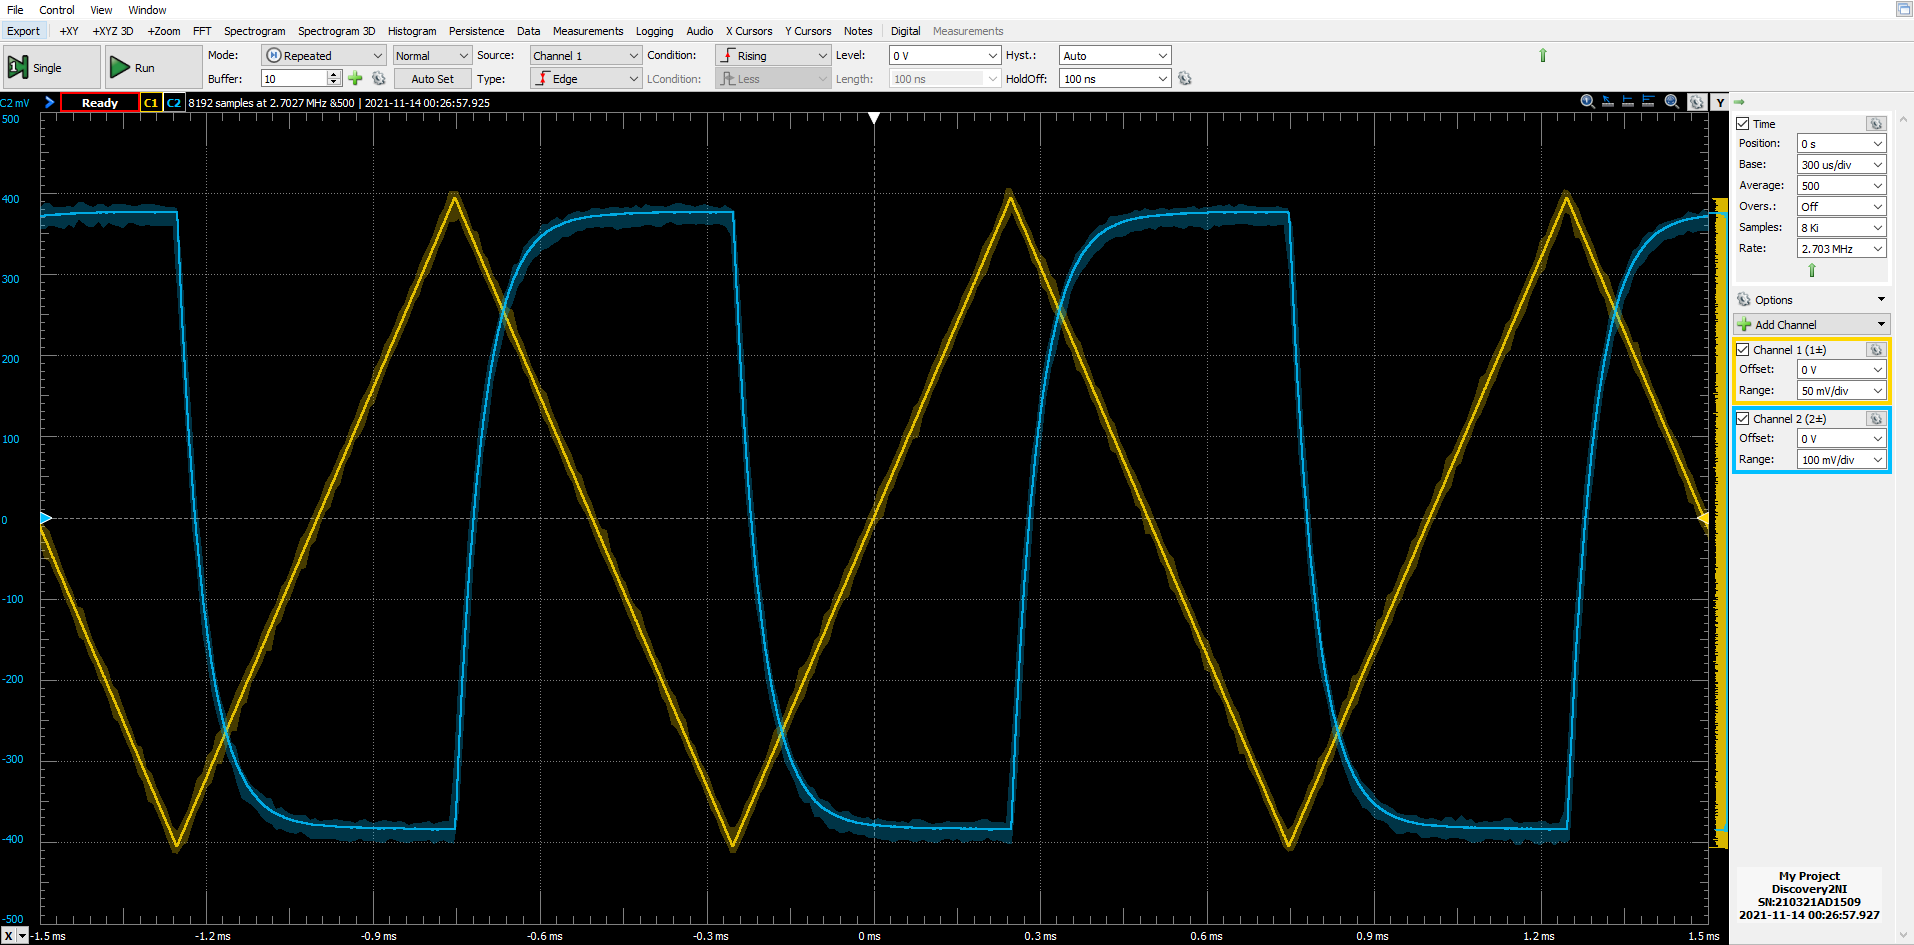
\includegraphics[scale=0.335]{derfin}
\caption{Onda a pinna di squalo in risposta ad un triangolo di ampiezza
$200 \pm 2 \; \si{m\V}$ e $f = 1000 \pm 16 \; \si{Hz}$ in ingresso al
circuito derivatore. \label{fig: derfin}}
\end{figure}

Per frequenze $f \gg f_A$ il filtro torna in regime di taglio, ma ora si
comporta grosso modo come un integratore, infatti la forma d'onda in uscita è
costituita da una serie di parabole con concavità rivolte verso l'alto e verso
il basso con ampiezza sempre minore all'aumentare della frequenza.
\begin{figure}[htbp]
\centering
%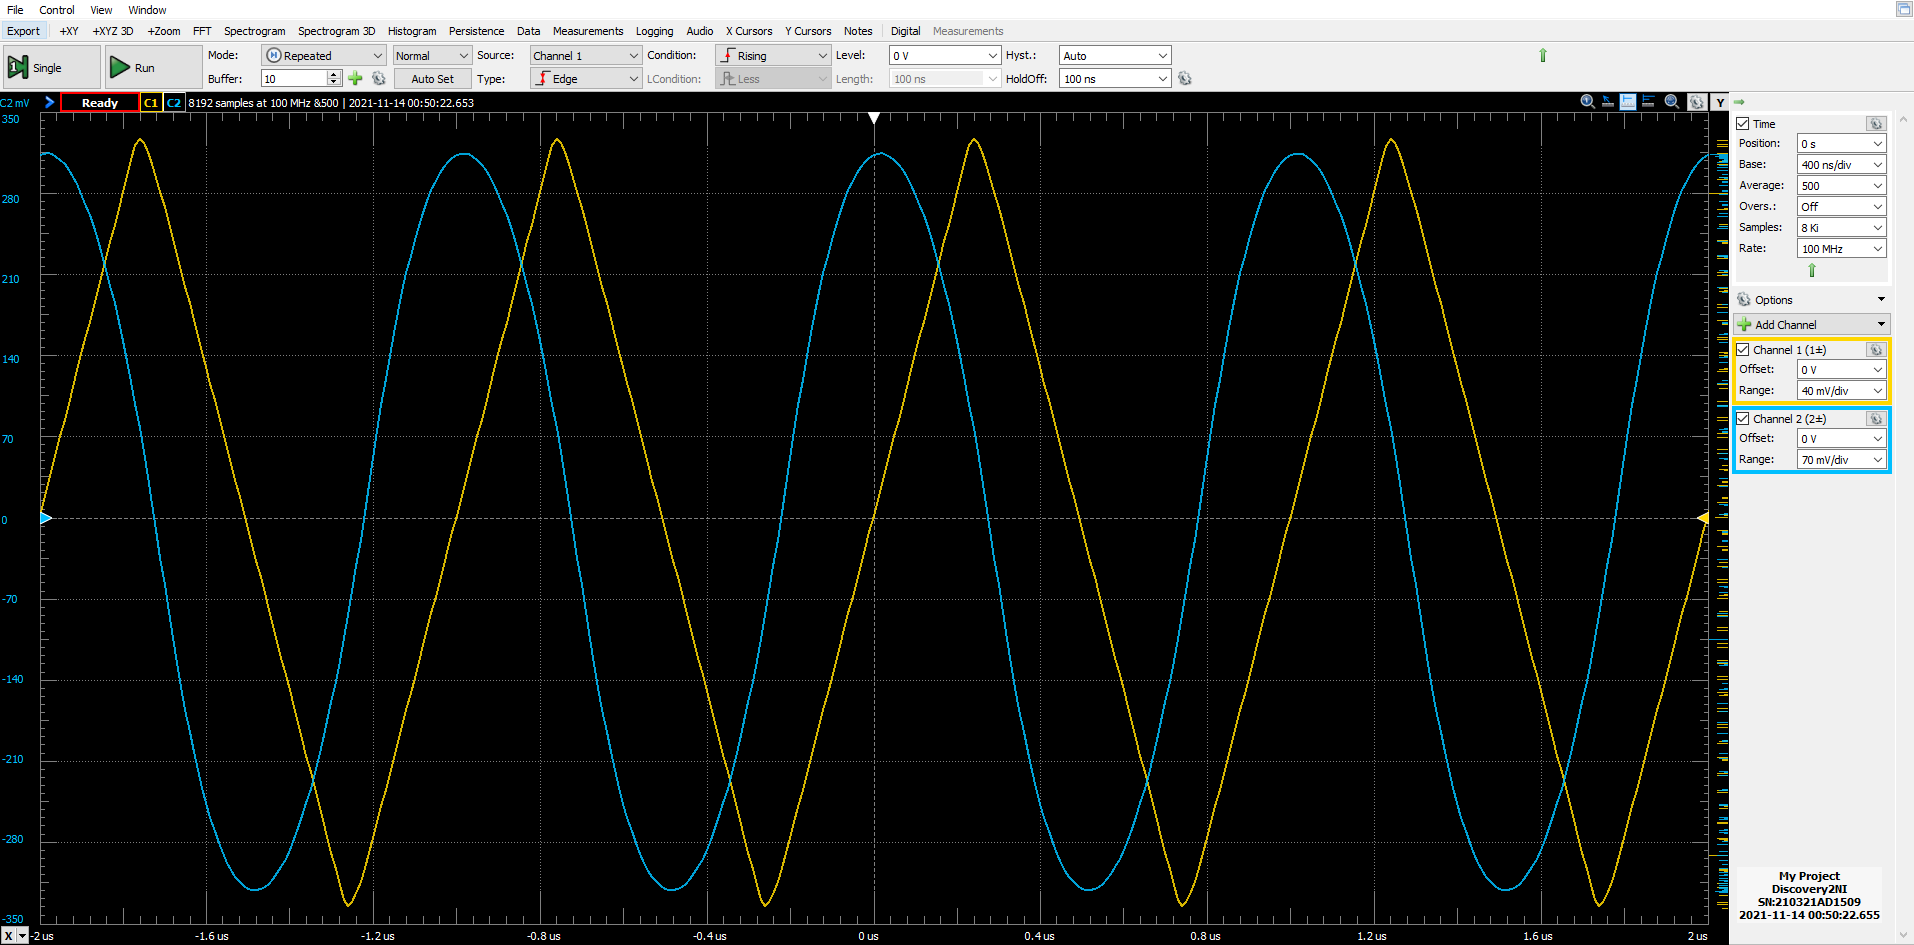
\includegraphics[scale=0.335]{derpar}
\caption{Parabole con concavità alternanti in risposta ad un triangolo di
ampiezza $200 \pm 2 \; \si{m\V}$ e $f = 1.00 \pm 0.02 \; \si{M\Hz}$ in ingresso
al circuito derivatore. \label{fig: derpar}}
\end{figure}

Inserendo tra l'uscita e la massa una resistenza di carico $R_L$ dello stesso
ordine di $R\ped{out}$ e misurando la tensione di uscita con o senza
resistenza è possibile dare una stima della resistenza in uscita
dell'amplificatore.
Detta $V_1$ la tensione misurata senza $R_L$ e $V_2$ la tensione misurata
con $R_L$, vale la formula:
\begin{equation}\label{eq: Zout}
\frac{R\ped{out}}{R_L} = \frac{V_1}{V_2} -1
\end{equation}
Per cui, una volta misurate $V_1 = 1725 \pm 8 \; \si{m\V}$,
$V_2 = 866 \pm 4\; \si{m\V}$ e $R_L = 5.08 \pm 0.05 \si{k\ohm}$ abbiamo 
ottenuto come impedenza d'uscita:
\[
R\ped{out} = R_L \left(\frac{V_1}{V_2} - 1\right)
\]

Risulta $R\ped{out} = 5.0 \pm 0.1\; \si{k\ohm}$ che è compatibile con la stima 
iniziale dell'impedenza.

\subsection{Misure di periodo e duty cycle}

\subsection{Limite massimo in frequenza del generatore}

%=======================
\section{Multivibratore monostabile}
\begin{figure}[htbp]
    \centering
	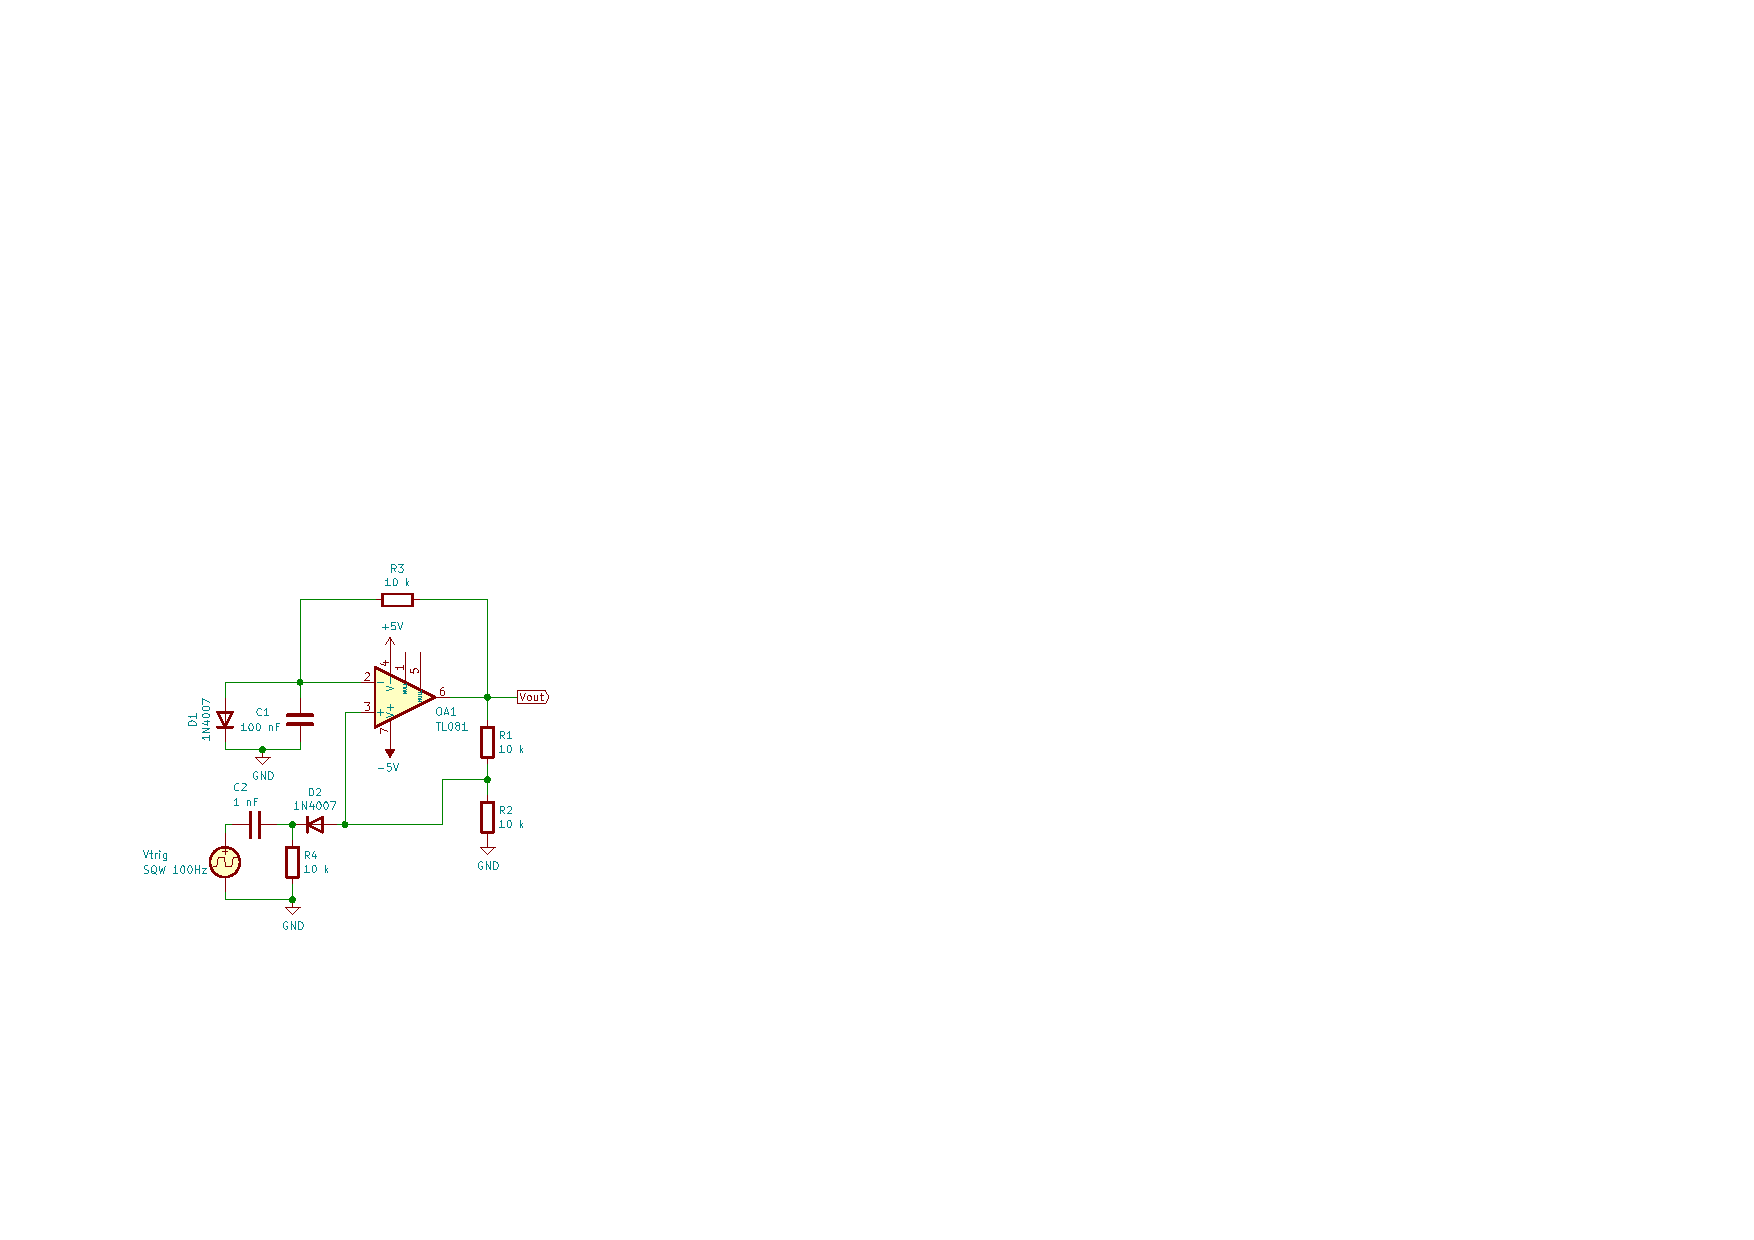
\includegraphics[scale=1.2]{monostable}
    \caption{Schema circuitale del multivibratore monostabile costruito.
    \label{fig: monostableschm}}
\end{figure}

\subsection{Studio dei segnali in ingresso e uscita}
Di nuovo utilizzando i cursori abbiamo misurato come guadagno a centro banda
per il circuito integratore attivo $A_M = 19.92 \pm 0.09 \; \si{dB}$.

Dunque abbiamo ricavato una stima della frequenza di taglio dell'amplificatore
invertente dal punto in cui il guadagno diminuisce di $-3.01 \; \si{dB}$
rispetto ad $A_M$:
$f_c = 342.5 \pm 0.5 \; \si{\Hz}$
\begin{figure}[htbp]
\centering
%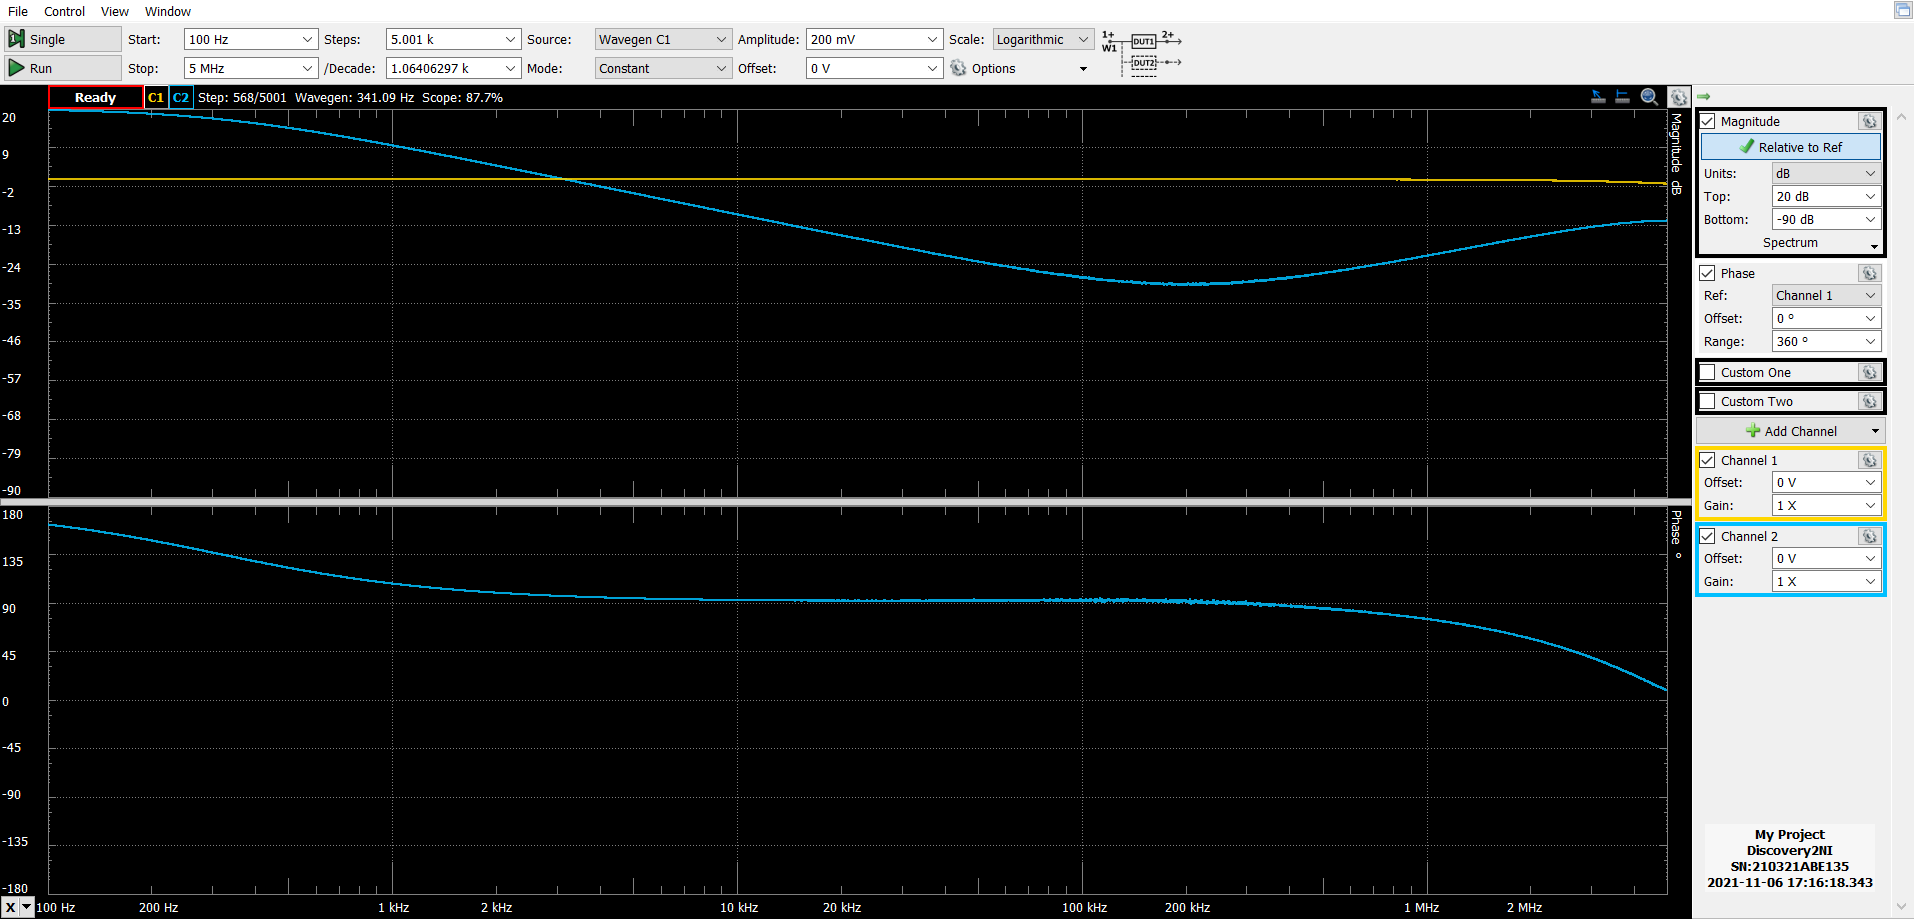
\includegraphics[scale=0.42]{bode integratore}
\caption{Plot di Bode ottenuto dallo scan con Network tra $\SI{10}{\Hz}$ e
$\SI{5}{M\Hz}$ con un segnale sinusoidale in ingresso all'integratore RC
attivo di ampiezza costante $v\ped{in} = \SI{200}{m\V}$.
\label{fig: intbode}}
\end{figure}

\subsection{Durata dell'impulso generato}
Si è inviato all'ingresso del filtro passa-basso un'onda quadra di
ampiezza $v\ped{in} = \SI{200}{m\V}$ e frequenza $10.02 \pm 0.12 \; \si{k\Hz}$.

$$v\ped{in} = 200 \pm 2 \; \si{m\V}$$
$$v\ped{out} = 107.3 \pm 1.3 \; \si{m\V}$$
$$A_v = \frac{v\ped{out}}{v\ped{in}} = 0.537 \pm 0.008$$

\begin{figure}[htbp]
\centering
%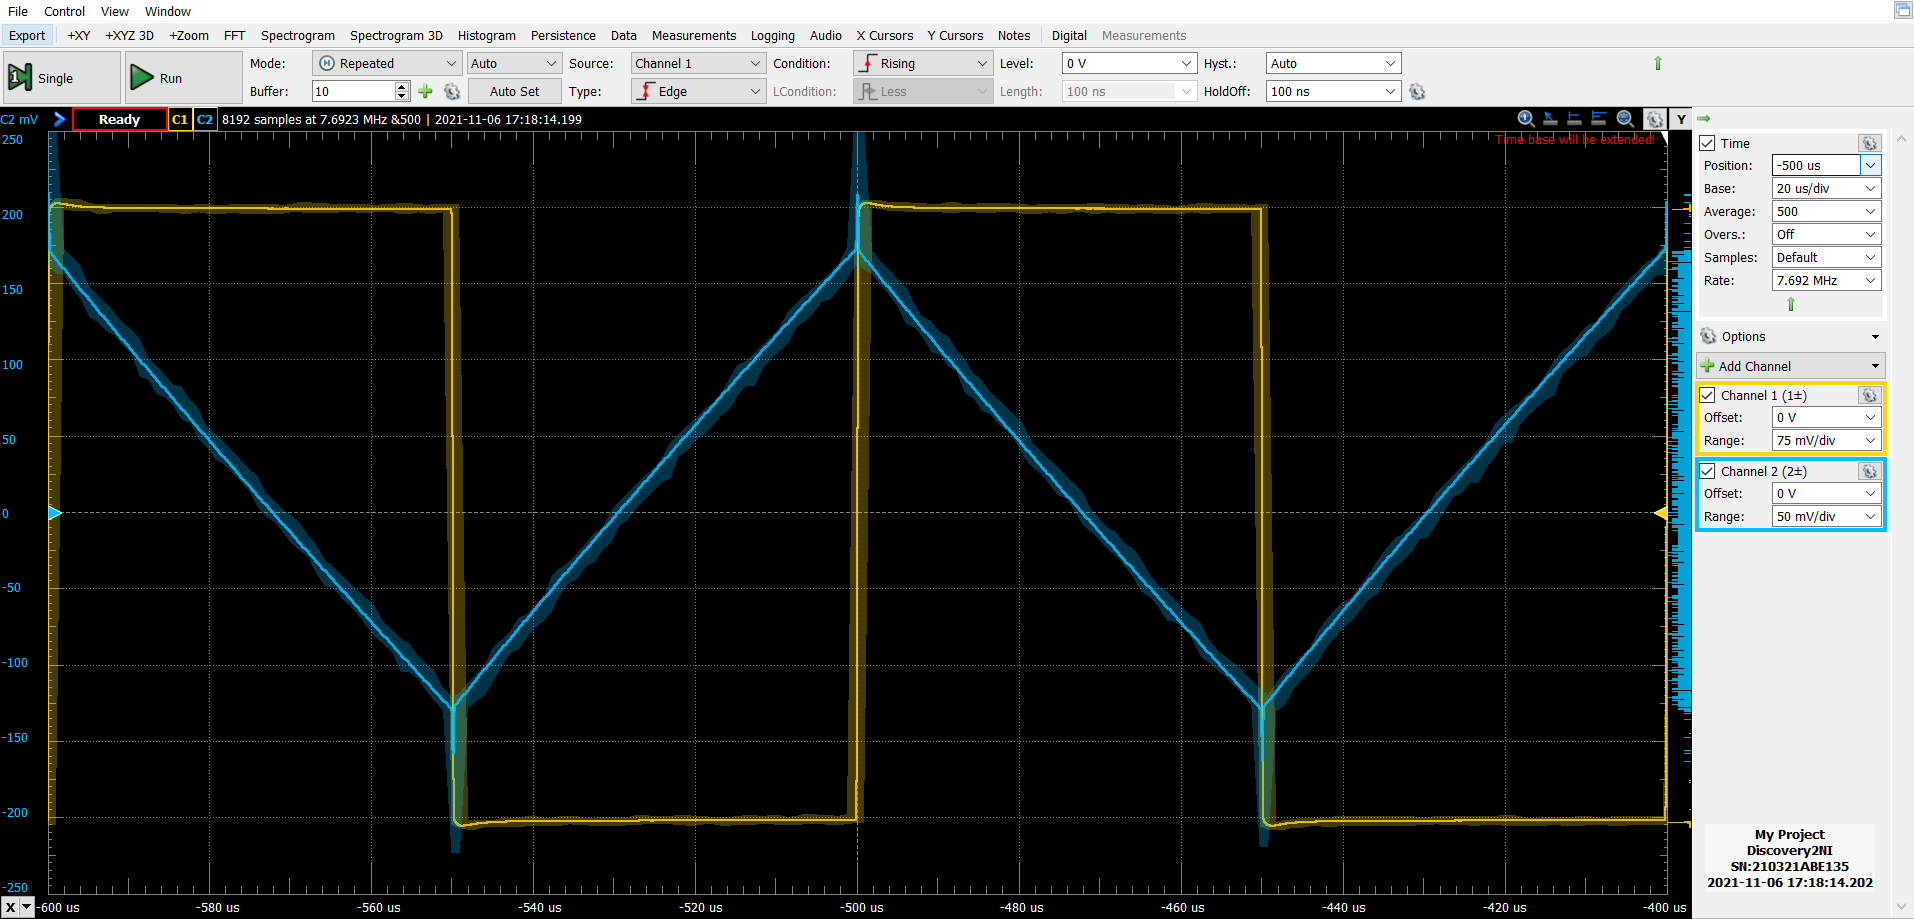
\includegraphics[scale=0.42]{integratore}
\caption{Risposta del circuito ad un'onda quadra di ampiezza
$\SI{200}{m\V}$ e $f = \SI{10}{k\Hz}$ in ingresso. \label{fig: intsqw}}
\end{figure}

Partendo da una misura con i cursori del guadagno a centro banda,
$A_V = 19.65 \pm 0.05 \; \si{dB} = 9.65 \pm 0.08$, possiamo ottenere una stima 
del valore
delle frequenze di taglio a bassa $f_L$ e ad alta frequenza $f_H$ dai punti
in cui il guadagno diminuisce di un fattore $1/\sqrt{2}$, cioè di circa
$-3.01 \; \si{dB}$ rispetto ad $A_V$.
\begin{align*}
f_L &= 80.77 \pm 0.12 \; \si{\Hz}\\
f_H &= 646.1 \pm 0.5 \; \si{k\Hz}
\end{align*}

Trascurando le capacità delle giunzioni nel transistor ci aspettiamo che
la frequenza di taglio ``bassa'' corrisponda a quella di un filtro passa~alto
costituito dalla serie $C\ped{in} + R_B$
\begin{equation}
f\ped{L, exp} = \frac{1}{2\pi R_B C\ped{in}} = 83 \pm 4 \; \si{\Hz}
\end{equation} 
che è in accordo con il valore misurato.

Mentre per la frequenza di taglio ``alta'' la resistenza in uscita è data
da $R_C$, per cui la capacità in serie dev'essere dell'ordine delle centinaia
di pF per avere ordine di grandezza compatibile con il valore misurato.
Ma nel datasheet risulta al massimo $C\ped{ibo} \approx \SI{25}{p\F}$, per cui
è difficile stabilire un valore di riferimento per la frequenza $f_H$ attesa.

Per frequenze $f \ll f_c$ come è ragionevole aspettarsi, la forma d'onda in
uscita non è apprezzabilmente cambiata rispetto all'onda quadra in ingresso,
ma risulta soltanto amplificata in ampiezza di un fattore $A_M \sim 10$.

Per frequenze $f \gg f_c$ il filtro è in regime di taglio, per cui si comporta
come un integratore, dunque la forma d'onda in uscita è un'onda triangolare di
ampiezza sempre minore al crescere della frequenza.

Nel regime intermedio $f \sim f_c$ all'uscita del filtro RC osserviamo un'onda
"a pinna di squalo" che corrispondono alle curve di carica e scarica del
condensatore al passaggio da basso ad alto e viceversa dell'onda quadra in
ingresso.
\begin{figure}[htbp]
\centering
%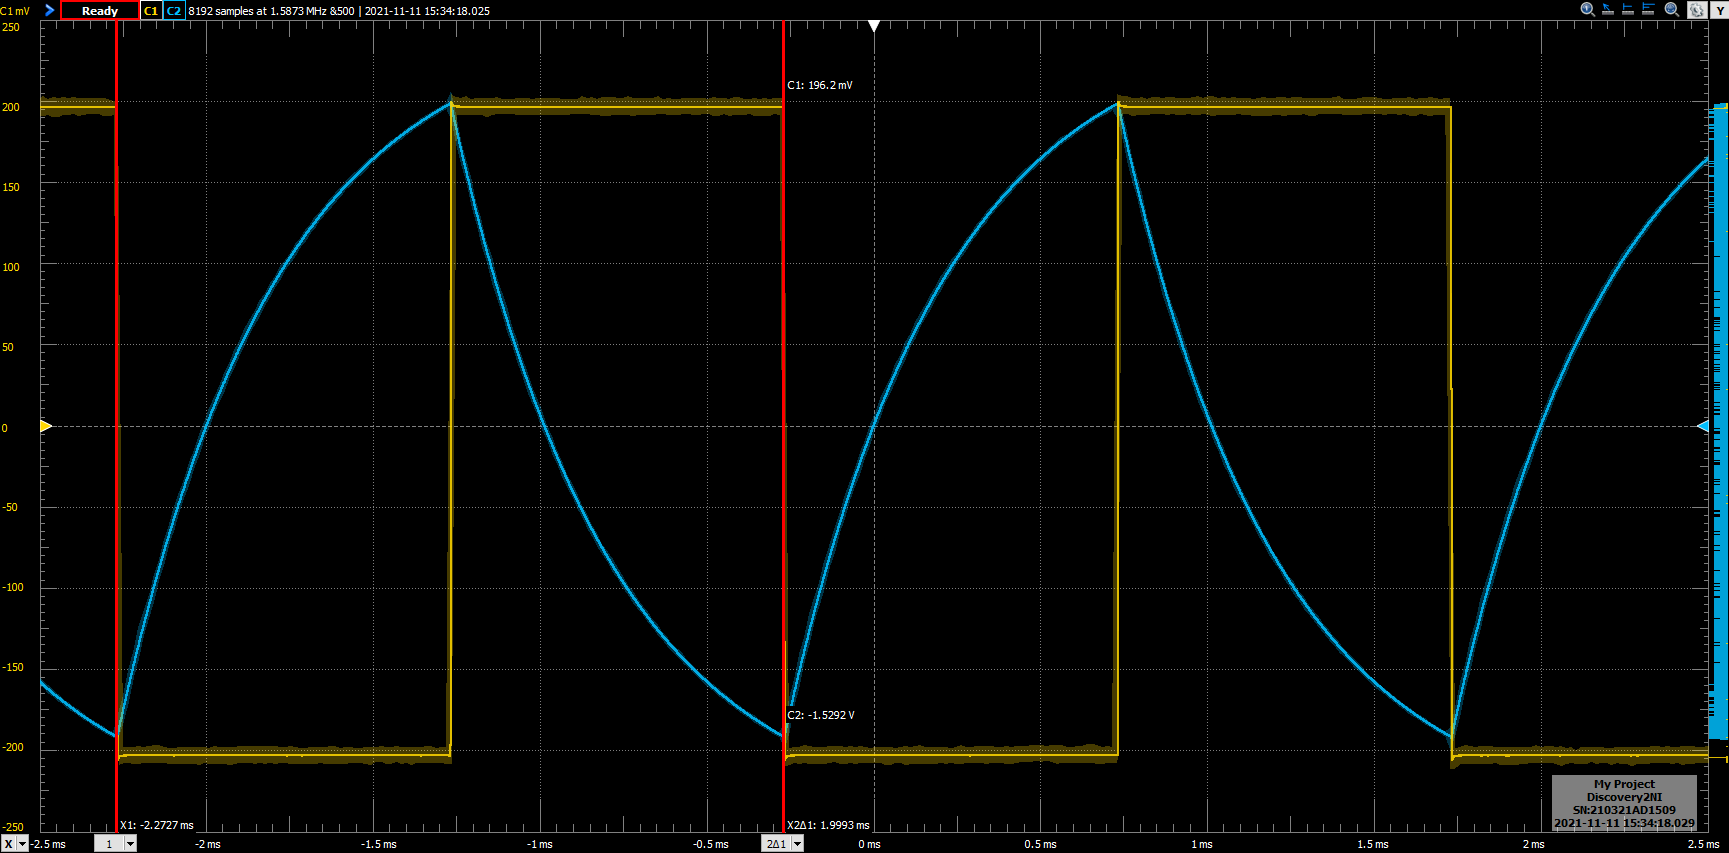
\includegraphics[scale=0.335]{intfin}
\caption{Onda a pinna di squalo in risposta ad un'onda quadra di ampiezza
$\SI{200}{m\V}$ e $f = 500 \pm 6 \; \si{Hz}$ in ingresso al circuito
integratore. \label{fig: intfin}}
\end{figure}

\subsection{Analisi del funzionamento del circuito}

%=======================
\section*{Conclusioni e commenti finali}
Si è riusciti a costruire e studiare alcuni dei circuiti più comuni che si
possono realizzare con un amplificatore operazionale, tra cui: due filtri
attivi, passa-basso e passa-alto, un amplificatore di tensione invertente
(e uno non).
In particolare siamo riusciti ad apprezzare il differente comportamento dei
circuiti (anche in regime non lineare) dare una stima di guadagno, impedenza di
ingresso e frequenze caratteristiche della loro risposta in frequenza.

%=======================
\section*{Dichiarazione}
I firmatari di questa relazione dichiarano che il contenuto della relazione \`e
originale, con misure effettuate dai membri del gruppo, e che tutti i firmatari
hanno contribuito alla elaborazione della relazione stessa.

\end{document}
